\chapter{Superfluidità}
L'elio $\ce{He}$ è un elemento abbastanza particolare appartenente ai gas nobili e scoperto nel 1868 dall'astronomo francese Jensen durante un'eclissi solare in India. Nel 1893 l'elio venne riscoperto da Ramsey sulla Terra, indipendentemente da Cleve e Langlet durante i loro studi su un minerale oggi noto come clevite che presentava la caratteristica di emettere nuclei di $\ce{^4He}$ a causa dei decadimenti $\alpha$ degli isotopi contenuti in esso. L'elio venne liquefatto per ultimo tra tutti i gas nobili nel 1908 da Kamerlingh nel suo laboratorio a Leiden. Le caratteristiche principali di questo elemento sono:
\begin{enumerate}
    \item a temperatura ambiente l'elio è un gas molto leggero ed inerte;
    \item è il secondo elemento più abbondante nell'Universo dopo l'idrogeno;
    \item gli isotopi stabili sono il bosone $\ce{^4He}$ con isospin $I = 0$ e il fermione $\ce{^3He}$ con isospin $I = 1/2$;
    \item gli isotopi instabili sono l'$\ce{^6He}$ con un'emivita $t_{1/2} \simeq \SI{0.82}{\second}$ e l'$\ce{^8He}$ con un'emivita $t_{1/2} \simeq \SI{0.12}{\second}$;
    \item è così leggero che sfugge all'attrazione gravitazionale terrestre, la stragrande maggioranza di quello presente sulla Terra proviene da isotopi che decadono $\alpha$.
\end{enumerate}
L'atomo di elio presenta simmetria sferica dato che possiede il primo orbitale elettronico completo, per questo è anche privo di un momento magnetico permanente. Il potenziale interatomico è tipicamente approssimato empiricamente con il potenziale di Lennard-Jones
\begin{equation}
\label{eq: potenziale Lennard - Jones}
    \phi(r) = 4\epsilon\bigg[\bigg(\frac{\sigma}{r}\bigg)^{12} - \bigg(\frac{\sigma}{r}\bigg)^6\bigg],
\end{equation}
dove il termine $\propto r^{-12}$ descrive l'azione repulsiva a corto raggio, mentre il termine $\propto r^{-6}$ descrive quella attrattiva dovuta alle forze dipolo-dipolo di van der Waals. Anche se non ha un momento magnetico permanente, l'elio è sempre soggetto a fluttuazioni di punto-zero, in particolare $\epsilon/k \simeq \SI{10.2}{\kelvin}$ e $\sigma \simeq \SI{2.56}{\angstrom}$. L'energia associata al potenziale $\phi(r)$ è data da
\begin{equation}
    U = \frac{1}{2}\int_0^\infty dr\,4\pi r^2\phi(r)n(r) \simeq \frac{A}{V_m^4} - \frac{B}{V_m^2},
\end{equation}
dove $n(r)$ è la densità radiale degli atomi di elio e $V_m$ è il volume molare. Dal grafico \ref{fig: He U(T) senza E0} di $U$ in funzione di $V_m$ sembrerebbe che l'elio non solidifichi nel limite in cui $T \to \SI{0}{\kelvin}$. Per capire se le cose stanno effettivamente così si devono includere gli effetti quantistici che dominano alle basse temperature. 
\begin{figure}[h]
    \centering
    \begin{subfigure}[t]{0.4\linewidth}
        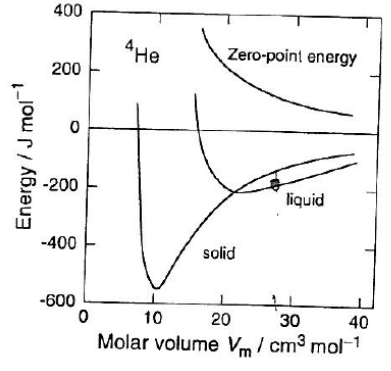
\includegraphics[width=0.9\linewidth]{Immagini - Capitolo 1/He U(T) senza E0.png}
        \caption{energia potenziale $U$ in funzione di $T$ dell'elio-4 senza $E_0$.}
        \label{fig: He U(T) senza E0}
    \end{subfigure}
    \hspace{0.1pt}
    \begin{subfigure}[t]{0.4\linewidth}
        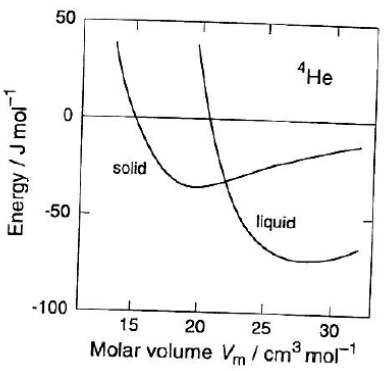
\includegraphics[width=0.9\linewidth]{Immagini - Capitolo 1/He U(T) con E0.png}
        \caption{energia potenziale $U$ in funzione di $T$ dell'elio-4 con $E_0$.}
        \label{fig: He U(T) con E0}
    \end{subfigure}
\end{figure}

Si consideri una particella racchiusa in una buca di potenziale infinita di lunghezza $L$, le energie accessibili al sistema sono
\begin{equation}
    E_n = \frac{\hbar^2\pi^2}{2mL^2}\sum_{i=1}^3(n_i+1)^2,
\end{equation}
quindi l'energia di punto zero è 
\begin{equation}
    E_0 = \frac{3\hbar^2\pi^2}{2mV^{2/3}} \simeq \frac{1}{V^{2/3}}.
\end{equation}
Quindi, a $T = \SI{0}{\kelvin}$ a pressione atmosferica è la fase liquida ad essere più stabile con un volume molare di circa $\SI{28}{\centi\meter\cubed\mol^{-1}}$, come mostrato in figura \ref{fig: He U(T) con E0}. In tabella \ref{tab: parametri del 3He e 4He} sono riportati alcuni parametri caratteristici dell'elio-3 e dell'elio-4.
\begin{table}[h]
    \centering
    \begin{tabular}{|c|cc|}
         \hline 
         & $\ce{^3He}$ & $\ce{^4He}$ \\ \hline
         temperatura di ebollizione a $\SI{1}{\atm}$ $[\mathrm{K}]$ & 3.19 & 4.21 \\
         temperatura critica $[\mathrm{K}]$ & 3.32 & 5.19 \\
         pressione critica $[\mathrm{bar}]$ & 1.16 & 2.29 \\
         densità per $T \to 0$ $[\SI{}{\gram\per\centi\meter\cubed}]$ & 0.076 & 0.145 \\
         densità al punto di ebollizione $[\SI{}{\gram\per\centi\meter\cubed}]$ & 0.055 & 0.125 \\ \hline
    \end{tabular}
    \caption{alcuni importanti parametri dell'elio-3 e dell'elio-4.}
    \label{tab: parametri del 3He e 4He}
\end{table}

Onnes scopre che la densità dell'$\ce{^4He}$ è eccezionalmente bassa e osserva che presenta un massimo intorno alla temperatura di $\SI{2}{\kelvin}$, come mostrato nel grafico in figura \ref{fig: He rho(T)}.
\begin{figure}[h]
    \centering
    \begin{subfigure}[t]{0.4\linewidth}
        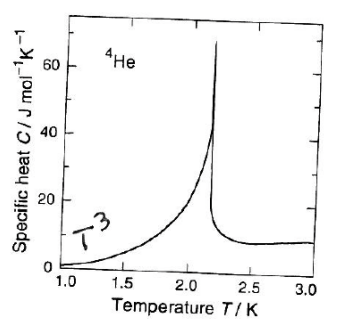
\includegraphics[width=0.9\linewidth]{Immagini - Capitolo 1/He c(T).png}
        \caption{andamento del calore specifico $c$ dell'elio-4 in funzione di $T$.}
        \label{fig: He c(T)}
    \end{subfigure}
    \begin{subfigure}[t]{0.4\linewidth}
        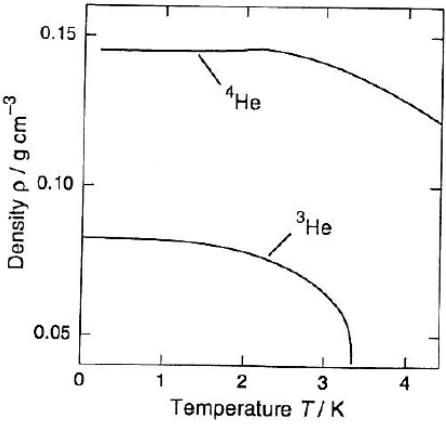
\includegraphics[width=0.9\linewidth]{Immagini - Capitolo 1/He rho(T).png}
        \caption{diagramma $p(T)$ dell'elio-4.}
        \label{fig: He rho(T)}
    \end{subfigure}
\end{figure}
Nel 1923 Dana ed Onnes osservano sperimentalmente che il calore specifico dell'elio-4 cresce vertiginosamente sempre intorno ai $\SI{2}{\kelvin}$, sempre mostrato in figura \ref{fig: He c(T)}, ma il fatto fu inizialmente attribuito ad un problema sperimentale dovuto alle difficoltà tecniche dell'esperimento. Tuttavia, nel 1932 con il miglioramento della tecnologia, Keesam e Clausius confermarono la validità della scoperta di Onnes e Dana alla temperatura $T_\Lambda = \SI{2.17}{\kelvin}$. Poiché la natura della transizione rimaneva sconosciuta, per molto tempo le due fasi dell'elio vennero battezzate con i nomi di elio-I per $T > T_\Lambda$ e elio-II per $T < T_\Lambda$. Il motivo per cui la temperatura di transizione è indicata con $T_\Lambda$ è che l'andamento della curva del calore specifico in funzione di $T$ ricorda la forma della lettera greca in questione. Il punto di transizione venne infatti denominato ``$\Lambda$-point''. 
\begin{obs}
    Inizialmente, si pensava che l'elio-II fosse una fase ``solida'' del tipo cristallo liquido.
\end{obs}
Al contrario di ciò che si pensava inizialmente il calore specifico non tende ad infinito, invece è approssimabile con una funzione a tratti
\begin{equation}
    c_V = 
    \begin{cases}
        c(T) + A_+|T - T_\Lambda|^{-\alpha},\quad T > T_\Lambda \\
        c(T) + A_-|T - T_\Lambda|^{-\alpha},\quad T < T_\Lambda
    \end{cases},\quad \alpha = 0.009,
\end{equation}
dove $c(T)$ è una funzione continua. La transizione quindi è del secondo ordine in quanto 
\begin{equation}
    S = -\frac{\p G}{\p T}\bigg|_p,\quad c_V = -T\frac{\p^2G}{\p T^2}\bigg|_p
\end{equation}
sono funzioni continue. Sempre Dana ed Onnes osservarono che il calore latente di vaporizzazione $L$ ha un minimo intorno ai $\SI{0.8}{\kelvin}$ e tende a crescere per temperature ancora minori. Il diagramma delle fasi $p(T)$ dell'elio-4 è riportato in figura \ref{fig: He p(T)}. Partendo dall'energia libera di Gibbs si ha che all'equilibrio le energie della fase solida e liquida si equivalgono, per cui 
\begin{equation}
\label{eq: equilibrio fase liquida e solida elio-4}
    G_{l} \simeq G_s\quad\Longrightarrow\quad \mu_l \simeq \mu_s.
\end{equation}
\begin{figure}[h]
    \centering
    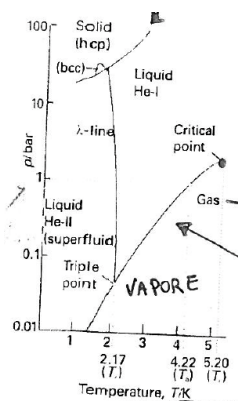
\includegraphics[width=0.25\linewidth]{Immagini - Capitolo 1/He p(T).png}
    \caption{grafico $p(T)$ dell'elio-4.}
    \label{fig: He p(T)}
\end{figure}

Adesso conoscendo le equazioni di stato $\p_TG = - S$ e $\p_pG = V$ si può espandere l'espressione \eqref{eq: equilibrio fase liquida e solida elio-4} ottenendo
\begin{align}
    \frac{\p G_l}{\p T}\delta T + \frac{\p G_l}{\p p}\delta p &= \frac{\p G_s}{\p T}\delta T + \frac{\p G_s}{\p p}\delta p \\
    V_l\delta p - S_l \delta T &= V_s\delta T - S_s\delta p,
\end{align}
da cui, riarrangiando i termini, si trova l'equazione di Clausius-Clapeyron
\begin{equation}
\label{eq: equazione di Clausius-Clapeyron}
    \frac{dp}{dT} = \frac{S_s - S_l}{V_s - V_l} = \frac{\Delta S}{\Delta V}.
\end{equation}
Dato che $V_l > V_s$ se $dp/dT < 0$ per $T < \SI{0.8}{\kelvin}$, allora $S_s > S_l$. Quindi, l'entropia del solido di $\ce{^4He}$ è maggiore di quella della fase liquida. 

Una delle caratteristiche più importanti dell'elio-II è la proprietà di passare attraverso capillari senza essere oggetto della forza d'attrito. Questa proprietà di superfluidità venne scoperta da Kapitza, e indipendentemente da Allen e Misener. Per spiegare la natura di questa proprietà, nel 1938 London suggerisce sia legata alla condensazione di Bose-Einstein. Adottando questo punto di vista, Tisza formula un modello fenomenologico ``a due fluidi''. Quando la temperatura tende a zero, la lunghezza d'onda di de Broglie $\lambda$ diventa paragonabile alla distanza interatomica e gli atomi perdono la loro identità comportandosi come onde. 
\begin{figure}[h]
    \centering
    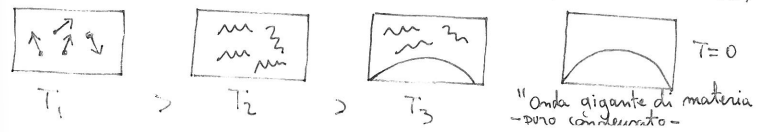
\includegraphics[width=0.9\linewidth]{Immagini - Capitolo 1/comportamento ondulatorio atomi.png}
    \caption{evoluzione verso un comportamento ondulatorio degli atomi del condensato.}
    \label{fig: comportamento ondulatorio atomi}
\end{figure}

Infatti, se la lunghezza d'onda di de Broglie è  $\lambda = h/p$, con il fatto che $p=mv$ e tramite il teorema di equipartizione dell'energia che restituisce la relazione 
\begin{equation}
    \frac{1}{2}m\vmedio{v^2} = \frac{3}{2}kT
\end{equation}
si può definire la lunghezza di de Broglie termica come
\begin{equation}
    \lambda_T = \frac{h}{\sqrt{3mkT}}.
\end{equation}
Per $T = \SI{300}{\kelvin}$ si ha che $\lambda_T = \SI{e-8}{\centi\meter}$, mentre per $T = \SI{e-8}{\kelvin}$ si trova $\lambda_T = \SI{e-3}{\centi\meter}$. A temperature $T > T_\Lambda$ l'elio liquido si comporta come un gas molto denso, ma a $T = T_\Lambda$ quasi tutte le proprietà dell'elio cambiano drasticamente. Seguendo la linea di ebollizione si ha che l'elio si comporta come come un fluido normale, ossia che è soggetto ad ebollizione, mentre a temperature minori di $T_\Lambda$ questo smette di bollire. Questo è dovuto al fatto che la capacità termica diventa cinque ordini di grandezza più grande di quella dell'elio-I. Dunque, in generale non è possibile impostare un gradiente di temperatura in un superfluido, come non è possibile impostare una differenza di potenziale ai capi di un conduttore ideale con resistenza nulla. Inoltre, l'elio per $T < T_\Lambda$ non ha viscosità. Esiste anche un altro effetto detto ``meccano-calorico''. Dati due recipienti contenenti elio alla stessa temperatura e pressione collegati da un capillare molto sottile a $T < T_\Lambda$, come mostrato in figura \ref{fig: esperimento capillare}, se si incrementa la pressione $p_A$, allora il livello in $A$ si abbassa e quello in $B$ si alza, come ci si aspetta per un fluido incomprimibile.
\begin{figure}[h]
    \centering
    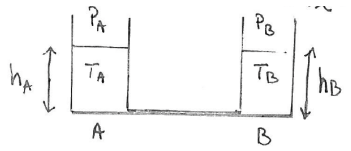
\includegraphics[width=0.5\linewidth]{Immagini - Capitolo 1/esperimento capillare.png}
    \caption{esperimento del capillare.}
    \label{fig: esperimento capillare}
\end{figure}
Tuttavia, corrispondentemente la temperatura in $B$ si abbassa, mentre quella in $A$ aumenta, pertanto attraverso il capillare passa solamente la componente superfluida a $S = 0$. Esiste anche l'effetto inverso detto ``termomeccanico''. Nella medesima situazione, se si aumenta la temperatura di $A$ si osserva una differenza di livello nei due recipienti, in particolare $h_A > h_B$. Nell'esperimento del beaker si osserva come l'elio supefluido possieda una tensione superficiale non nulla; infatti, l'elio in questa fase riesce ad arrampicarsi fuori dalle pareti di un contenitore per ottenere l'equilibrio chimico pur avendo viscosità nulla. Inoltre, nell'elio-II si osservano delle onde di temperatura che si propagano ad una velocità caratteristica, ciò è dovuto all'enorme capacità termica. Poiché la propagazione avviene in modo molto simile a quanto si osserva con le onde sonore, questo effetto è stato rinominato come ``secondo suono''. Tutte queste proprietà derivano dal ``modello a due fluidi'' di Tisza.

\section{Modello a due fluidi}
L'idea è di considerare l'elio-II come composto da un insieme di due fluidi completamente interpenetranti con proprietà diverse. Anche se questa interpretazione non è totalmente corretta\footnote{Infatti, non è possibile che nell'elio-II vi siano atomi appartenenti ad un fluido normale ed altri appartenenti ad un superfluido: gli atomi sono indistinguibili e la funzione d'onda totale deve essere simmetrica per lo scambio di particelle.}, il modello gode di un discreto successo. Si supponga quindi che la densità dell'elio-II si possa separare in due contributi dovuti al fluido normale e al superfluido rispettivamente, in tal caso
\begin{equation}
    \rho_{\ce{^4He}} = \rho_N(T) + \rho_S(T),
\end{equation}
dove i due termini dipendono dalla temperatura $T$. A $T = \SI{0}{\kelvin}$ l'elio-II è composto unicamente dal superfluido e $\rho_N = 0$, invece per $T \ge T_\Lambda$ è presente solo la componente ordinaria e $\rho_S  = 0$.
\begin{figure}[h]
    \centering
    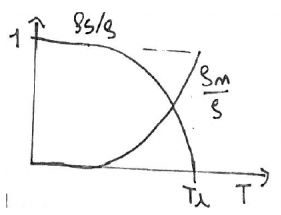
\includegraphics[width=0.3\linewidth]{Immagini - Capitolo 1/He rhoS(T).png}
    \caption{andamento di $\rho_S/\rho$ in funzione di $T$.}
    \label{fig: He rhoS(T)}
\end{figure}
La densità $\rho$ dipende anche dalla temperatura, ma le fluttuazioni nel range che si sta considerando sono minime. Nel caso dei bosoni liberi si ha che $\rho_S = \rho_0 = 0$, mentre nel caso dell'elio la situazione è complicata a causa dell'interazione intermolecolare; infatti, gli atomi perdono la loro identità e sono le eccitazioni collettive che diventano importanti. Anche a $T = \SI{0}{\kelvin}$ si ha $\rho_N \neq \rho_S$, per cui non tutte le particelle rimangono nello stato con $\vk = 0$, portando al fenomeno della deplezione quantistica. Conviene quindi identificare $\rho_N$ con la densità di eccitazioni collettive. Si noti che il calore specifico $c_V$ nell'elio-II a $T \simeq \SI{0}{\kelvin}$ cresce come $T^3$ e il sistema si comporta come un gas di fononi non interagenti.
\begin{table}[h]
    \centering
    \begin{tabular}{|c|ccc|}
         \hline
         componente & densità & viscosità & entropia \\ \hline
         normale & $\rho_N$ & $\eta_N \neq 0$ & $S_N \neq 0$ \\
         superfluida & $\rho_S$ & $\eta_S = 0$ & $S_S = 0$ \\ \hline
    \end{tabular}
    \caption{caratteristiche delle componenti normale e superfluida dell'$\ce{^4He}$.}
    \label{tab: caratteristiche componenti 4He}
\end{table}

\subsection{Effetto termomeccanico}
L'effetto termomeccanico è una conseguenza dell'equazione \eqref{eq: equazione di Clausius-Clapeyron} ottenuta imponendo $d\mu = 0$ all'equilibrio. Si supponga di avere due contenitori $A$ e $B$ con $\ce{^4He}$ a $T < T_\Lambda$. I contenitori sono completamente isolati, ossia adiabatici e rigidi, ma collegati tra loro da un capillare che fa passare solo la componente superfluida. Se non avvengono processi irreversibili, l'entropia totale $S$ del sistema $A + B$ è costante, come mostrato in figura \ref{fig: effetto termomeccanico}.
\begin{figure}[h]
    \centering
    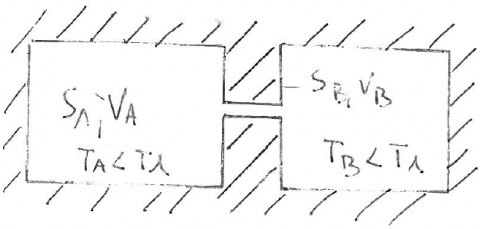
\includegraphics[width=0.4\linewidth]{Immagini - Capitolo 1/effetto termomeccanico.png}
    \caption{sistema isolato contenente elio-4 a $T < T_\Lambda$.}
    \label{fig: effetto termomeccanico}
\end{figure}
Poiché attraverso il capillare può solo passare la componente superfluida con $S = 0$, allora anche l'entropia all'interno dei due contenitori è costante, per cui $S_A$ e $S_B$ sono costanti. Si denota con $U_T$ l'energia interna totale e con $U_l$, dove $l = \{A,B\}$, l'energia interna per unità di massa definita come 
\begin{equation}
    U_T = \sum_{l=A,B}M_lu_l,
\end{equation}
dove $M_l$ è la massa di $\ce{^4He}$ nel rispettivo contenitore. All'equilibrio termodinamico l'energia interna totale è minima, quindi 
\begin{equation}
    \delta U_T = \sum_{l=A,B}(u_l\delta M_l + M_l\delta u_l) = 0.
\end{equation}
Poiché anche l'entropia $S_l$ è costante, quindi 
\begin{equation}
\label{eq: variazione entropia s_l}
    \delta S_l = s_l\delta M_l + M_l\delta s_l = 0 \quad\Longrightarrow\quad \delta s_l = -s_l\frac{\delta M_l}{M_l}.
\end{equation}
Il volume $V_l = M_lv_l$ è anche costante, per cui
\begin{equation}
\label{eq: variazione volume v_l}
    \delta v_l = -v_l\frac{\delta M_l}{M_l}.
\end{equation}
Sviluppando ora $\delta u_l(s,v)$ si trova
\begin{equation}
    \delta u_l = \frac{\p u}{\p s_l}\bigg|_{v_l}\delta s_l + \frac{\p u}{\p v_l}\bigg|_{s_l}\delta v_l,
\end{equation}
con il quale ponendo si ricava
\begin{equation}
    \delta U_T = \nsum_l\bigg[u_l\delta M_l + M_l\bigg(\frac{\p u}{\p s_l}\bigg|_{v_l}\delta s_l + \frac{\p u}{\p v_l}\bigg|_{s_l}\delta v_l\bigg)\bigg] = 0,
\end{equation}
ma sapendo che 
\begin{equation}
    \frac{\p u}{\p s}\bigg|_v = T,\quad \frac{\p u}{\p v}\bigg|_s = -p,
\end{equation}
si arriva a 
\begin{equation}
    \nsum_l[u_l\delta M_l + M_l(T_l\delta s_l - p_l\delta v_l)] = 0
\end{equation}
dove sostituendo le relazioni \eqref{eq: variazione entropia s_l} e \eqref{eq: variazione volume v_l} si trova
\begin{equation}
    \nsum_l(u_l - s_lT_l + v_lp_l)\delta M_l = \nsum_l \mu_l \delta M_l = 0,
\end{equation}
ma se la massa è conservata $\delta M_A = - \delta M_B$ e quindi si trova la condizione di equilibrio chimico
\begin{equation}
    \mu_A(T_A,p_A) = \mu_B(T_B,p_B).
\end{equation}
Anche per $T_A \neq T_B$ si raggiunge l'equilibrio $\mu_A = \mu_B$ attraverso lo scambio di atomi ad entropia nulla, modificando quindi anche $p_A$ e $p_B$. Se $T_A = T_B + \delta T$ e $p_A = p_B + \delta p$, allora sviluppando al primo ordine $\mu_A$ si ottiene
\begin{equation}
    \frac{\p\mu_A}{\p T_A}\delta T + \frac{\p \mu_A}{\p p_A}\delta p = 0,
\end{equation}
da cui si ricava l'equazione di London 
\begin{equation}
\label{eq: equazione di London}
    \delta p = \frac{s_A}{v_A}\delta T.
\end{equation}
Dunque, se aumenta la differenza di temperatura, aumenta proporzionalmente la differenza di pressione a causa di un flusso di atomi della componente superfluida che attraversa il capillare dal contenitore $B$ ad $A$. L'effetto termomeccanico si può osservare anche nell'esperimento della fontanella. Come mostrato in figura \ref{fig: esperimento fontanella}, l'elio è riscaldato nella zona del gomito da un fascio molto tenue di luce. Dell'elio superfluido entra nel tubo attraverso il filtro capillare per mantenere il potenziale chimico, ma questo fa aumentare il livello dell'elio nel tubo verticale che fuoriesce dall'apertura superiore creando una fontanella. Attraverso il filtro capillare si instaura quindi un flusso spontaneo dal contenitore ``freddo'' all'interno del tubo ``caldo''. Poiché il superfluido dal contenitore non trasporta entropia, questo processo non viola il secondo principio della Termodinamica. Fontanelle stazionarie di circa $\SI{30}{\centi\meter}$ sono state ottenute in questo modo. Di solito il flusso è turbolento, ma in certe condizioni le fontanelle possono esserne prive. 
\begin{figure}[h]
    \centering
    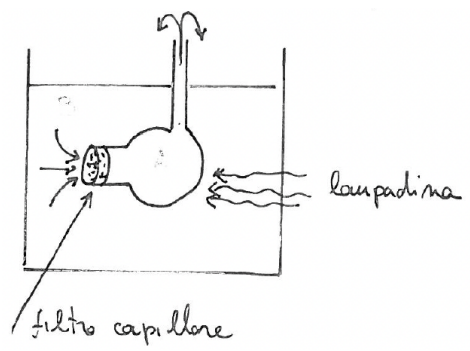
\includegraphics[width=0.4\linewidth]{Immagini - Capitolo 1/esperimento fontanella.png}
    \caption{esperimento della fontanella.}
    \label{fig: esperimento fontanella}
\end{figure}

La spiegazione del comportamento stranormale dell'elio liquido nell'esperimento del beaker può essere spiegato utilizzando i potenziali chimici. Considerando il diagramma in figura \ref{fig: esperimento beaker}, l'elio forma una pellicola sottile sulla superficie del recipiente sopra il livello dell'elio liquido. La pellicola si forma a causa dell'interazione di van der Waals tra gli atomi di elio e le pareti del contenitore. All'equilibrio si ha 
\begin{equation}
\label{eq: condizione equilibrio esperimento beaker}
    \mu_{film}(z) = \mu_{vap} = \mu_l(z = 0) \equiv \mu_l(0).
\end{equation}
Poiché si sono forze esterne come quella di van der Waals e la gravità, questi sono i potenziali chimici totali, con $\mu_{film}$ corrispondente alla somma di tre termini
\begin{equation}
    \mu_{film}(z) = \mu_l(0) + \mu_g(z) + \mu_{vdW}(z) = \mu_l(0) \Longrightarrow \mu_g = gz = - \mu_{vdW},
\end{equation}
dove si è usata la \eqref{eq: condizione equilibrio esperimento beaker}. 
\begin{figure}[h]
    \centering
    \begin{subfigure}[t]{0.4\linewidth}
        \centering
        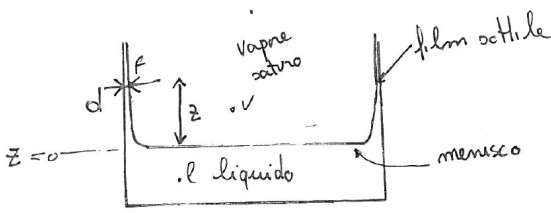
\includegraphics[width=0.95\linewidth]{Immagini - Capitolo 1/esperimento beaker.png}
        \caption{esperimento del beaker.}
        \label{fig: esperimento beaker}
    \end{subfigure}
    \begin{subfigure}[t]{0.4\linewidth}
        \centering
        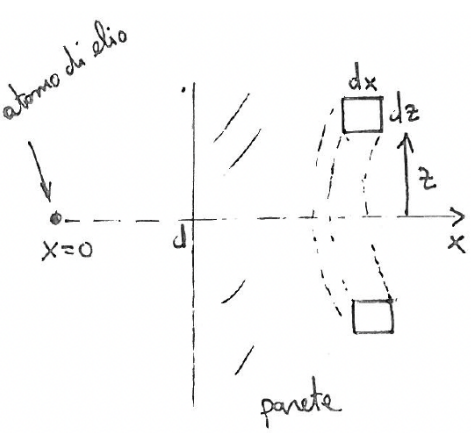
\includegraphics[width=0.7\linewidth]{Immagini - Capitolo 1/esperimento beaker (calcolo).png}
        \caption{costruzione per l'esperimento del beaker.}
        \label{fig: esperimento beaker (calcolo)}
    \end{subfigure}
\end{figure}

Il potenziale chimico di van der Waals si ottiene integrando il potenziale $\phi(r) \propto -1/r^6$. Lo spessore della parete è dell'ordine del millimetro, quindi molto più grande delle distanze interatomiche, per cui è approssimabile ad uno spessore infinito. Si divide quindi lo spazio nella parete di destra in corone circolari con sezione $dx$ per $dz$ e raggio $z$, come mostrato in figura \ref{fig: esperimento beaker (calcolo)}. Quindi, 
\begin{equation}
    \begin{split}
        \mu_{vdW} \propto -\int_d^\infty dx\int _0^\infty dz\, \frac{2\pi z}{(z^2 + x^2)^3} &\overset{y=z^2}{=} -\int_d^\infty dx \int _0^\infty dy\,\frac{\pi}{(x^2 + y^2)^3} \\
        &= -\int_d^\infty dx\,\bigg[\frac{-\pi}{2}(x^2 + y^2)^{-2}\bigg]_0^\infty \\
        &= -\frac{\pi}{2}\int_d^\infty \frac{dx}{x^4} \\
        &= -\frac{\pi}{6d^3}.
    \end{split}
\end{equation}
Dunque, $\mu_{vdW} = -\alpha/d^3$ dove $\alpha$ è la costante di Hamaker. In totale da $\mu_g = gz = -\alpha/d^3$ si ha l'equazione del menisco
\begin{equation}
\label{eq: equazione del menisco}
    d = \sqrt[3]{\frac{\alpha}{gz}}.
\end{equation}
La costante $\alpha$ è ottenuta a partire dalle proprietà dielettriche dell'elio e dalle pareti del recipiente misurate sperimentalmente. All'equilibrio in condizione di vapore saturo si trova che a $z = \SI{10}{\centi\meter}$ lo spessore del film è $d \simeq \SI{200}{\angstrom}$. Un fluido normale non potrebbe scorrere in un capillare di queste dimensioni. Le proprietà superfluida dell'elio non sono importanti per determinare lo spessore del film ma lo sono per perché scorrere all'interno del film senza attrito. L'elio superfluido si diffonde su tutte le pareti per minimizzare il potenziale chimico ovunque. 

\subsection{Secondo suono}
Le variazioni di temperatura in un sistema omogeneo si propagano nel mezzo in accordo con l'equazione di propagazione del calore
\begin{equation}
\label{eq: equazione di propagazione del calore}
    \nabla^2 T = \frac{1}{D}\frac{\p }{\p t}T(\vx,t).
\end{equation}
Nell'elio-II la conducibilità termica $D$ è infinita, quindi l'equazione precedente non è più valida. Si può pensare che il membro di destra dell'equazione \eqref{eq: equazione di propagazione del calore} sia in realtà il primo termine di uno sviluppo in serie di Taylor in $t$: se il primo termine è zero, il termine successivo con la derivata seconda non è più trascurabile; perciò ci si aspetta che l'equazione venga modificata nel modo seguente
\begin{equation}
    \nabla^2 T = \frac{1}{v}\frac{\p^2 T}{\p t^2},
\end{equation}
che rappresenta la propagazione per onde delle variazioni di temperatura. Dunque. nell'elio-II ci si aspettano due tipi di propagazione per onde:
\begin{enumerate}
    \item il suono, ossia la propagazione di onde di pressione o densità descritte dall'equazione di d'Alembert $\square\rho = 0$, dove $\rho_N$ e $\rho_S$ sono indistinguibili e oscillano in fase;
    \item il secondo suono, ossia la propagazione di onde termiche, legate a fluttuazioni di $\rho_N$ a $\rho$ costante, dove $\rho_N$ e $\rho_S$ oscillano in opposizione di fase.
\end{enumerate}
Una variazione locale di $\rho_N$ corrisponde ad una variazione locale della temperatura, quindi il secondo suono è un'onda di temperatura. Nell'ambito del modello a due fluidi è facile derivare l'equazione di propagazione del secondo suono nel caso del gas di fononi (elio-II a $T \simeq \SI{0}{\kelvin}$). Si indica con $u = U/V$ l'energia per unità di volume del gas di fononi. L'equazione della meccanica $\vF = m\va$ per un fluido si traduce in 
\begin{equation}
    \frac{d\vq}{dt} = -\nabla p,
\end{equation}
dove $\vq$ è la quantità di moto per unità di volume. D'altra parte, l'equazione di continuità per l'energia è
\begin{equation}
    \frac{1}{v_1^2}\frac{d u}{dt} + \nabla \cdot \vq = 0,
\end{equation}
da cui si ha
\begin{equation}
    \frac{\p ^2u}{\p t^2} = v_1^2\nabla^2 p.
\end{equation}
Tuttavia, per un gas di fononi la pressione $p$ è legata alla densità di energia da 
\begin{equation}
    p = - \frac{\p F(T,V)}{\p V}\bigg|_T,\quad F(T,V,N) = U(S,V,N) - \frac{\p U}{\p S}S,
\end{equation}
quindi sapendo anche che
\begin{equation}
    F = -\frac{U}{3} = -\frac{\sigma VT^4}{3},
\end{equation}
dove $\sigma$ nel caso del corpo nero sarebbe la costante di Stefan-Boltzmann, si ha
\begin{equation}
    p = \frac{\sigma T^4}{3} = \frac{u}{3}.
\end{equation}
Quindi, si ottiene
\begin{equation}
    \frac{\p ^2 u}{\p t^2} - \frac{v_1^2}{3}\nabla^2 u = 0
\end{equation}
e dunque la velocità del secondo suono è 
\begin{equation}
    v_2 = \frac{v_1}{\sqrt{3}}.
\end{equation}
Le fluttuazioni della densità dei fononi si propagano con una velocità caratteristica pari a $v_2 \simeq \SI{137}{\meter\per\second}$ a $T = \SI{0}{\kelvin}$, ma per problemi tecnici, questo valore limite per $T < \SI{0.5}{\kelvin}$ non è ancora stato confermato dagli esperimenti. Le fluttuazioni in $u$ sono legate a quelle in $T$ dal fatto che $\delta u \propto \bar{T}^3\delta T$.
\begin{figure}[h]
    \centering
    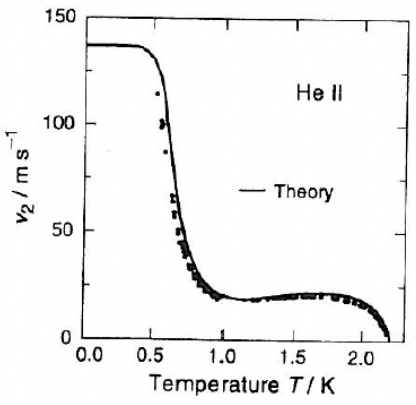
\includegraphics[width=0.35\linewidth]{Immagini - Capitolo 1/He v2(T).png}
    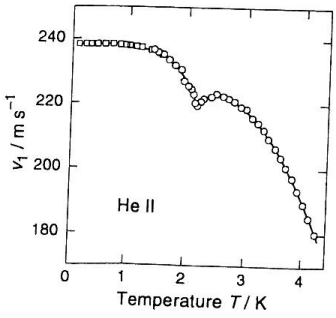
\includegraphics[width=0.35\linewidth]{Immagini - Capitolo 1/He v1(T).png}
    \caption{andamento in funzione di $T$ del: (i) primo suono $v_1$; (ii) secondo suono $v_2$.}
    \label{fig: He v1(T) e v2(T)}
\end{figure}

\subsection{Velocità critica}
Dopo aver discusso il fenomeno del secondo tramite la verifica della propagazione di onde di temperatura ad una velocità caratteristica, si passa ad analizzare una proprietà fondamentale dei superfluidi: avere viscosità nulla. La viscosità è la manifestazione macroscopica dello scambio di energia tra un fluido in scorrimento e la parte lungo cui scorre. Poiché questo scambio avviene per quanti, dove le eccitazioni sono quasi-particelle, può succedere che per ragioni cinematiche un fluido a $T = \SI{0}{\kelvin}$ che scorre a velocità inferiore ad un valore critico non possa produrre quasi-particelle nell'interazione con la parete, non perdendo quindi energia ed avendo allora viscosità nulla. Il tutto dipende dalla relazione di dispersione che lega l'energia $\epsilon$ all'impulso $\vq$ delle quasi-particelle. Nell'elio superfluido, la diffusione inelastica con fasci di neutroni permette di stabilire che la curva di dispersione ha approssimativamente la forma mostrata in figura \ref{fig: He e(q)}. Per piccoli valori di $q$, ossia per grandi lunghezze d'onda, si ha $\epsilon(q) = v_1 q$, dove $v_1$ è la velocità del primo suono a $T = \SI{0}{\kelvin}$. Eccitazioni di questo tipo sono i quanti del suono, cioè i fononi. Queste sono le eccitazioni più importanti per il comportamento termico del fluido a $T < \SI{0.5}{\kelvin}$. Al di sopra di questa temperatura entra in gioco un altro tipo di quasi-particella, il rotone, corrispondete al minimo locale nella curva di dispersione. Si cercano ora i vincoli cinematici per la produzione di una particella con impulso $\vq$ ed energia $\epsilon(q)$ da parte di un fluido di massa $M$ che scorre lungo una parete con velocità $\vv$. Per la conservazione dell'impulso e per la conservazione dell'energia si hanno
\begin{equation}
    \begin{cases}
        M\vv = M\vv' + \vq \\[1.5ex]
        \dfrac{1}{2}Mv^2 = \dfrac{1}{2}M(v')^2 + \epsilon(q)
    \end{cases}
\end{equation}
da cui, sostituendo $\vv' = \vv - \vq/M$ nella seconda equazione, si trova
\begin{equation}
    \vv \cdot \vq - \frac{q^2}{2M} = \epsilon(q).
\end{equation}
Considerando il limite in cui $M \to \infty$, si ottiene che
\begin{equation}
   \vv \cdot \vq = \epsilon(q)\quad\Longrightarrow\quad v > \frac{\epsilon(q)}{q},
\end{equation}
per cui esiste una velocità critica $v_c$ sotto la quale il fluido ha viscosità nulla data dalla velocità di London 
\begin{equation}
    v_c = \min_{q}\bigg\{\frac{\epsilon(q)}{q}\bigg\}.
\end{equation}
In conclusione, ogni sostanza che è liquida a $T = \SI{0}{\kelvin}$ ed ha uno spettro di eccitazioni formato, a bassa energia, da fononi è necessariamente un superfluido a tale temperatura perché esiste una velocità critica $v_c > 0$.
\begin{figure}[h]
    \centering
    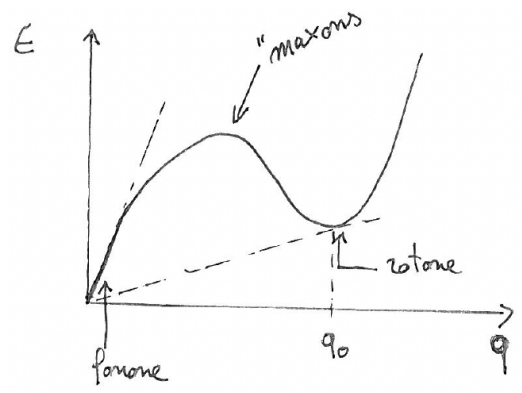
\includegraphics[width=0.35\linewidth]{Immagini - Capitolo 1/He e(q).png}
    \caption{andamento di $\epsilon$ in funzione di $q$ dell'elio superfluido.}
    \label{fig: He e(q)}
\end{figure}
\begin{obs}
    Per lungo tempo si pensò che la superfluidità fosse legata all'esistenza di un gap di energia, in analogia al fenomeno della superconduttività; tuttavia, ciò non è possibile a causa del fatto che i fononi possono avere un'energia arbitrariamente piccola.
\end{obs}
Per $T > \SI{0}{\kelvin}$ il ragionamento precedente continua a valere, ma adesso il liquido contiene un gas di fononi, o più in generale di quasi-particelle, che possono interagire con le pareti dando luogo ad un comportamento viscoso. Le velocità critiche sono 
\begin{equation}
    v_c(fononi) \simeq \SI{238}{\meter\per\second} \equiv v_1,\quad v_c(rotoni) \simeq \SI{60}{\meter\per\second} \equiv \frac{\epsilon(q_0)}{q_0}.
\end{equation}
Lo stesso Landau pensava che la velocità critica osservata negli esperimenti fosse determinata dai rotoni, tuttavia risulta invece che a pressione ambiente si possono creare vortici ad anello a velocità considerevolmente inferiore a quella critica dei rotoni. Nel gas di bosoni ideale si ha che l'energia è pari all'energia cinetica $\epsilon(q) = q^2/2m$, per cui la velocità critica è
\begin{equation}
    v_c = \min_q{\bigg(\frac{\epsilon(q)}{q}\bigg)} = \min_q{\bigg(\frac{q}{2m}\bigg)} = 0.
\end{equation}
Dunque, il gas di bosoni ideale non è un superfluido. L'interpretazione microscopica dei fononi e dei rotoni è molto diversa. A piccoli valori di $q$, un atomo di elio è fortemente accoppiato agli altri atomi del condensato e i fononi corrispondono alle tipiche onde di compressione e rarefazione nei fluidi e nei solidi. Per valori di $q$ molto grandi, le particelle si muovono quasi liberamente nel condensato e la curva di dispersione cresce come
\begin{equation}
    \epsilon(q) \simeq \frac{q^2}{2m^*} + \mu,\quad q \gg 0,
\end{equation}
dove $m^*$ è la massa efficace. Per valori intermedi dell'impulso, un atomo in movimento è fortemente accoppiato solo con i minimi vicini. Quando avanza, quelli che lo precedono si spostano lateralmente per poi passargli dietro; l'effetto netto è simile a quello di un anello vorticoso, come mostrato in figura \ref{fig: fononi e rotoni}. 
\begin{figure}[h]
    \centering
    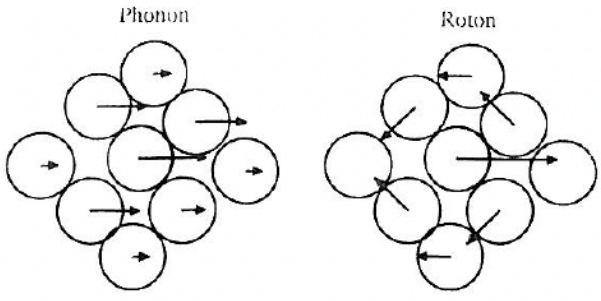
\includegraphics[width=0.4\linewidth]{Immagini - Capitolo 1/fononi e rotoni.png}
    \caption{comportamento dei fononi e dei rotoni.}
    \label{fig: fononi e rotoni}
\end{figure}

\section{Stato quantistico macroscopico}
L'equazione di Schr\"odinger che descrive un sistema di $N$ bosoni identici è
\begin{equation}
\label{eq: equazione di Schrodinger per un gas di bosoni}
    i\hbar\frac{\p}{\p t}\phi(\vr_1,\dots,\vr_N;t) = \hatH_N\phi(\vr_1,\dots,\vr_N;t),
\end{equation}
con hamiltoniana
\begin{equation}
\label{eq: hamiltoniana per un gas di bosoni}
    \hatH_N = \sum_{i=1}^N\bigg[-\frac{\hbar^2}{2m}\nabla^2 + V_{ext}(\vr_i)\bigg] + \frac{1}{2}\sum_{i\neq j}V(|\vr_i - \vr_j|),
\end{equation}
dove $\{\vr_i\}$ è l'insieme delle coordinate delle particelle, $V(|\vr_i - \vr_j|)$ è il potenziale interatomico e $V_{ext}(\vr_i)$ è il potenziale esterno. Dato che le particelle sono bosoni, la funzione d'onda deve essere simmetrica per lo scambio di particelle
\begin{equation}
\label{eq: simmetria per permutazioni della funzione d'onda di un gas di bosoni}
    \phi(\vr_1,\dots,\vr_i,\vr_j,\dots,\vr_N;t) = \phi(\vr_1,\dots,\vr_j,\vr_i,\dots,\vr_N;t).
\end{equation}
Nel caso in cui tutte le particelle siano nello stato fondamentale quantistico, per cui $N \to N_0$ a $T = \SI{0}{\kelvin}$, si può introdurre l'approssimazione di Hartree-Fock per cui la funzione d'onda si fattorizza secondo
\begin{equation}
\label{eq: approssimazione di Hartree-Fock per un gas di bosoni}
    \phi_0(\vr_1,\dots,\vr_{N_0}) = \prod_{i=1}^{N_0} \frac{\phi_0(\vr_i)}{\sqrt{N_0}},
\end{equation}
dove la funzione d'onda di singola particella è normalizzata con
\begin{equation}
\label{eq: normalizzazione funzione d'onda in approssimazione di Hartree-Fock}
    \int d^3r\,\phi_0^*(\vr)\phi_0(\vr) = \int d^3r\,\frac{\rho_S(\vr)}{m} = \int d^3r\,n_S(\vr) = N_0.
\end{equation}
Nell'approssimazione di Hartree-Fock lo stato quantistico macroscopico presente nell'elio-II e nel condensato di Bose-Einstein a $T = \SI{0}{\kelvin}$ può essere descritto dalla funzione d'onda
\begin{equation}
    \phi_0(\vr) = |\phi_0(\vr)|e^{i\theta(\vr)} = \sqrt{n_S(\vr)}e^{i\theta(\vr)}.
\end{equation}
La fase della funzione d'onda è legata alla velocità del superfluido; infatti, si può introdurre la densità di corrente
\begin{equation}
    \vj_S(\vr) = -\frac{i\hbar}{2m}(\phi_0^*\nabla\phi_0 - \phi_0\nabla\phi_0^*) = n_S(\vr)\frac{\hbar}{m}\nabla\theta(\vr) \equiv n_S(\vr)\vv_S(\vr).
\end{equation}
Quindi, si può determinare che la relazione tra la velocità e la fase è
\begin{equation}
    \vv_S = \frac{\hbar}{m}\nabla\theta(\vr),
\end{equation}
ma da questa si deduce immediatamente che la velocità è irrotazionale dato che il rotore di un gradiente è sempre nullo, per cui
\begin{equation}
    \nabla \times \vv_S(\vr) = 0.
\end{equation}
Dunque, in un superfluido non c'è turbolenza. La velocità della componente superfluida è determinata dalla fase della funzione d'onda: la fase è costante per $\vv_S = \vo$ e varia uniformemente per $\vv_S$ costante. Si possono pensare gli atomi di elio superfluidi come particelle che si comportano in modo coerente, una proprietà del tutto simile alla coerenza di fase nei laser. 

Landau propose un test per verificare l'irrotazionalità della componente superfluida dell'elio-II tramite un contenitore in rotazione. Si consideri la componente normale del contenitore in rotazione con velocità $v_N = \omega r$, per cui la forma della componente superfluida in rotazione è definita da una parabola
\begin{equation}
    z = \frac{\omega^2r^2}{2g} + h.
\end{equation}
Se si integra in una regione circolare $A_c$ di raggio $R$ centrata in $r = 0$ e si usa il teorema di Stokes assumendo che $\rho_S \neq 0$ ovunque in $A_c$ si ha
\begin{equation}
\label{eq: teorema di Stokes irrotazionalità elio-II}
    0 = \int_{A_c}(\nabla \times \vv_S)\cdot d\Sigma = \oint_C \vv_S\cdot d\vl = 2\pi R \vv_S,
\end{equation}
da cui si trova che $v_S = 0$, mentre $v_N = \omega R \neq 0$. Apparentemente la componente superfluida non può ruotare insieme a $\rho_N$, ma allora è a riposo? Nel caso in cui $\rho_S$ non partecipi alla rotazione, poiché la forza di gravità agisce su entrambe le componenti, il menisco dovrebbe appiattirsi per $T < T_\Lambda$ man mano che la temperatura diminuisce. Tuttavia, sperimentalmente Osborne non osserva nulla di tutto questo: il superfluido non è fermo ma partecipa alla rotazione. Il problema del risultato trovato in \eqref{eq: teorema di Stokes irrotazionalità elio-II} sta proprio nell'applicazione del teorema di Stokes e per vederlo si deve cambiare geometria considerando un contenitore toroidale; in tal caso la circuitazione è
\begin{equation}
    k = \oint_L \vv_S \cdot d\vl = \frac{\hbar}{m}\oint_L \nabla\theta(\vr)\cdot d\vl \equiv \frac{\hbar}{m}\delta\phi_L.
\end{equation}
Poiché la funzione d'onda $\psi(\vr)$ è ad un solo valore, la fase finale può differire da quella iniziale solo per multipli $\delta\phi_L = 2n\pi$, con $n \in \Z$, e si trova il teorema della circuitazione di Feynman
\begin{equation}
\label{eq: teorema della circuitazione di Feynman}
    k = \frac{\hbar}{m}2n\pi = \frac{hn}{m}.
\end{equation}
Essenzialmente, l'errore consisteva nell'assumere che il dominio $A_c$ dell'integrale di Stokes fosse semplicemente connesso.
\begin{figure}[h]
    \centering
    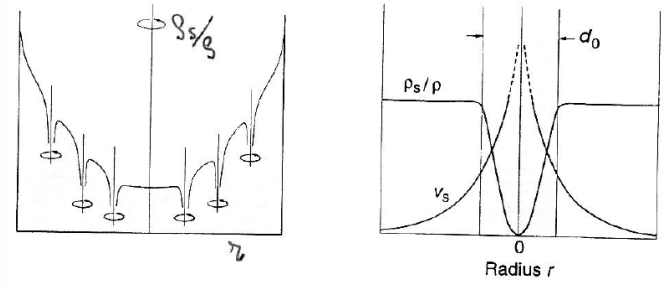
\includegraphics[width=0.7\linewidth]{Immagini - Capitolo 1/vortici He SF.png}
    \caption{formazione dei vortici nell'elio superfluido in rotazione.}
    \label{fig: vortici He SF}
\end{figure}
La conseguenza è che quando si ruota un superfluido si creano dei buchi, come mostrato in figura \ref{fig: vortici He SF}. Un vortice con simmetria cilindrica di questo tipo è descritto da un campo di velocità 
\begin{equation}
    \vv_S(\vr) = (v_x,v_y) = \frac{k}{2\pi r^2}(-y,x)\Rightarrow v_S = \frac{k}{2\pi r} = (\SI{1.58}{\meter\per\second})\times\frac{n}{r}.
\end{equation}
Si può stimare il diametro $d_0$ del nucleo del vortice ponendo
\begin{equation}
    v_S(d_0/2) \simeq v_c(rotone) \simeq \SI{60}{\meter\per\second}.
\end{equation}
In questo modo si trova un valore per $d_0$ dell'ordine di qualche angstrom, cioè dell'ordine delle distanze interatomiche. Il raggio del nucleo del vortice si chiama anche lunghezza di contrazione, che può crescere per $T \simeq T_\Lambda$. 

L'energia $E_v$ per unità di lunghezza di un vortice può essere calcolata integrando l'energia cinetica per unità di volume associata alla rotazione di $\rho_S$ 
\begin{equation}
    E_v = \int_{a_0}^b dr\,\frac{\rho_S v_S^2}{2}2\pi r,
\end{equation}
dove $a_0 \simeq d_0/2$ e $b$ è la metà della distanza tra i vortici o il raggio $R$ del recipiente in rotazione. Poiché $v_S = k/2\pi r$ con $k = nh/m$ si ha
\begin{equation}
    \begin{split}
        E_v = \int_{a_0}^b dr\,\frac{\rho_S k^2}{4\pi r} &= \frac{k^2\rho_S}{4\pi}\log{\frac{b}{a_0}} \\
        &= \frac{n^2h^2\rho_S}{4\pi m^2}\log{\frac{b}{a_0}} \\
        &= \pi n^2\rho_S\bigg(\frac{\hbar}{m}\bigg)^2\log{\frac{b}{a_0}},
    \end{split}
\end{equation}
da cui si vede che $E_v \propto n^2$ e la creazione di molti vortici con vorticità minima con $n = 1$ è energeticamente favorita rispetto, ad esempio, alla creazione di un unico vortice macroscopico centrale con vorticità $k = nh/m$. L'asse del vortice non è necessariamente una retta, ma una linea che può terminare sulle pareti del contenitore o richiudersi su se stessa dando origine a vortici ad anello. Questi vortici sono soluzioni ad energia finita delle equazioni del moto dell'elio superfluido. A causa della quantizzazione della circuitazione di $\vv_S$ queste soluzioni sono stabili e quindi non perdono energia per dissipazione. I vortici si possono creare attraverso l'introduzione di un eccesso di carica tramite elettroni, questi vengono intrappolati nel nucleo del vortice e tramite un campo elettrico si possono raccogliere sulla superficie. I vortici tendono a formare un reticolo triangolare detto ``reticolo di Abriskov''. Per capire come fa a formarsi un vortice quantizzato in un fluido irrotazionale, si può pensare di avere inizialmente due parti di superfluido separate da una sottile parete di fluido normale. Le due parti viaggiano parallele a velocità diverse. Sono due sistemi separati e le funzioni d'onda $\phi_A(x)$ e $\phi_B(x)$ differiscono di una fase. Si supponga che siano in fase a $x = 0$ per cui $\phi_A(0) = \phi_B(0) = \phi_0$, allora
\begin{equation}
    \phi_A(x) = \phi_0\exp{\bigg(\frac{i\hbar}{m}\int_0^x \vv_{S,A}\cdot d\vl\bigg)},\quad \phi_B(x) = \phi_0,
\end{equation}
quindi $\phi_A(x) = \phi_B(x)$ ogni volta che 
\begin{equation}
    \exp{\bigg(\frac{i\hbar}{m}\int_0^x \vv_{S,A}\cdot d\vl\bigg)} = e^{i2\pi n} = 1,
\end{equation}
ossia lungo i cammini chiusi in figura \ref{fig: circuiti He SF}. 
\begin{figure}
    \centering
    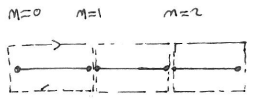
\includegraphics[width=0.4\linewidth]{Immagini - Capitolo 1/circuiti He SF.png}
    \caption{cammini chiusi percorsi dal superfluido.}
    \label{fig: circuiti He SF}
\end{figure}
La circuitazione lungo tali cammini è quantizzata e si può formare il vortice e il fluido normale all'interno può formare il suo nucleo. Vortici con vorticità opposta tendono a respingersi, mentre quelli con stessa vorticità tendono ad avvicinarsi dato che la pressione tra i due non è massima a causa della velocità non nulla del flusso tra i due. L'anello si muove in una direzione perpendicolare al suo piano ad una velocità $\vv_0$ di modulo
\begin{equation}
    v_0 = \frac{\hbar n}{2mr_0},\quad n \in \Z.
\end{equation}
Per ottenere questo valore, si ricorda che un vortice possiede un campo di velocità $v = k/2\pi r = \hbar/rm$ se si considera solo il caso $n = 1$, per cui considerando una sezione del vortice ad anello, come mostrato in figura \ref{fig: sezione toro He SF}, si ha
\begin{equation}
    v_A = \frac{2\hbar}{mr_0} - v_0,\quad v_B = \frac{\hbar}{mr_0} + v_0,
\end{equation}
quindi per non collassare il vortice ad anello deve muoversi verso il basso in modo che la velocità in $A$ e in $B$ siano uguali senza il verificarsi dell'effetto Magnus
\begin{equation}
    \frac{2\hbar}{mr_0} - v_0 = \frac{\hbar}{mr_0} + v_0 \Rightarrow v_0 = \frac{\hbar}{2mr_0}.
\end{equation}
\begin{figure}[h]
    \centering
    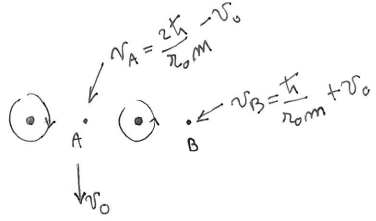
\includegraphics[width=0.5\linewidth]{Immagini - Capitolo 1/sezione toro He SF.png}
    \caption{sezione del vortice toroidale di elio superfluido.}
    \label{fig: sezione toro He SF}
\end{figure}

L'energia trasportata dal vortice si può calcolare approssimativamente applicando la formula del vortice a simmetria cilindrica per un anello di lunghezza $l = 2\pi r$ con
\begin{equation}
    \epsilon(r) = 2\pi r E_v(r) = \frac{k^2\rho_S}{2}r\log{\frac{r}{a_0}}.
\end{equation}
Quando l'elio scorre con velocità $\vv_S$ lungo un capillare di raggio $R$ può produrre dei vortici di raggio $r < R$ purché la valga la condizione di Landau
\begin{equation}
    v_S \ge v_c = \min_q\bigg\{\frac{\epsilon(q)}{q}\bigg\}.
\end{equation}
Per determinare l'impulso $q$ del vortice si usa il fatto che la derivata di $\epsilon(q)$ rispetto a $q$ coincide con la velocità di gruppo della corrispondente quasi-particella, quindi
\begin{equation}
    \frac{d\epsilon}{dq} = v = \frac{\hbar}{2mr},
\end{equation}
da cui 
\begin{equation}
    \frac{dq}{d\epsilon} = \frac{dq}{dr}\frac{dr}{d\epsilon} = \frac{2mr}{\hbar} \Rightarrow \frac{dq}{dr} = \frac{2mr}{\hbar}\frac{d\epsilon}{dr},
\end{equation}
ma d'altra parte si ha
\begin{equation}
    \frac{d\epsilon}{dr} = \frac{k^2\rho_S}{2}\log{\bigg(\frac{r}{a_0}\bigg)} + \frac{k^2\rho_S}{2} = \frac{k^2\rho_S}{2}\bigg[\log{\bigg(\frac{r}{a_0}\bigg)} + 1\bigg],
\end{equation}
che integrata tra $a_0 = d_0/2$ e la metà della distanza tra due vortici $r_0$ usando la relazione
\begin{equation}
    \int_0^r dx\,x\log{x} = \frac{1}{4}\int_0^r dx^2\,\log{x^2} = \frac{r^2}{2}\log{(r)} - \frac{r^2}{4},
\end{equation}
restituisce
\begin{equation}
    \begin{split}
        q &= \frac{k^2\rho_Sm}{\hbar}\int_{a_0}^{r_0}dr\,[r\log{(r)} + r(1 - \log{a_0})] \\
        &= \frac{k^2\rho_Sm}{\hbar}\bigg[\frac{r_0^2}{2}\log{(r_0)} - \frac{r_0^2}{4} - \frac{a_0^2}{2}\log{(a_0)} + \frac{a_0^2}{4} + \frac{r_0^2}{2} \\
        &- \frac{r_0^2}{2}\log{(a_0)} - \frac{a_0^2}{2} + \frac{a_0^2}{2}\log{a_0}\bigg] \\
        &= \frac{k^2\rho_Sm}{\hbar}\bigg[\frac{r_0^2}{2}\log{\bigg(\frac{r_0}{a_0}\bigg)} + \frac{r_0^2}{4} - \frac{a_0^2}{4}\bigg] \\
        &\simeq \frac{k^2\rho_Sm}{\hbar}\bigg[\frac{r_0^2}{2}\log{\bigg(\frac{r_0}{a_0}\bigg)} + \frac{r_0^2}{4}\bigg],
    \end{split}
\end{equation}
dove nell'ultimo passaggio si è trascurato il termine proporzionale a $a_0^2$ dato che $a_0 \ll 1$. Quindi, si ottiene
\begin{equation}
    \frac{\epsilon(r_0)}{q(r_0)} = \frac{\hbar}{mr_0}\frac{\log{(r_0/a_0)}}{\log{(r_0/a_0)} + 1/2} \overset{r_0 \gg a_0}{\simeq} \frac{\hbar}{mr_0},
\end{equation}
la quale ha un minimo per $r_0 \to R$, dunque la velocità critica è
\begin{equation}
    v_c = \frac{\hbar}{mR}\frac{\log{(R/a_0)}}{\log{(R/a_0)} + 1/2}.
\end{equation}
Si formano vortici ad anello delle dimensioni del capillare con una velocità di qualche $\mathrm{mm\,s^{-1}}$ in capillari di circa $\SI{1}{\milli\meter}$ di diametro. 

\subsection{L'equazione di Schr\"odinger non lineare}
L'equazione di Schr\"odinger a molti corpi associata al gas di bosoni è quella introdotta nell'equazione \eqref{eq: equazione di Schrodinger per un gas di bosoni} con hamiltoniana data da \eqref{eq: hamiltoniana per un gas di bosoni}, dove la funzione d'onda è simmetrica per permutazioni dei suoi argomenti come mostrato in equazione \eqref{eq: simmetria per permutazioni della funzione d'onda di un gas di bosoni}. Assumendo l'approssimazione di Hartree-Fock si ha un risultato simile a quello trovato in equazione \eqref{eq: approssimazione di Hartree-Fock per un gas di bosoni} dato da
\begin{equation}
    \phi(\vr_1,\dots,\vr_N) = \prod_{i=1}^N \frac{\phi(\vr_i,t)}{\sqrt{N}},
\end{equation}
con normalizzazione data da
\begin{equation}
    \int d^3r\,\phi^*(\vr,t)\phi(\vr,t) = N.
\end{equation}
La differenza è che adesso tutte le particelle non sono necessariamente nello stato fondamentale, anche se effettivamente l'idea è quella che $\phi(\vr,t)$ descriva solo la componente superfluida e che quindi $N \equiv N_0$ e $\phi(\vr,t) \equiv \phi_0(\vr,t)$. Si definisce l'energia media del sistema come
\begin{equation}
    E = \int d^3r_1\cdots d^3r_N\,\phi^*(\vr_1,\dots,\vr_N)\hatH_N\phi(\vr_1,\dots,\vr_N) = T + V_{ext} + V.
\end{equation}
Quindi, si calcolano 
\begin{equation}
    \begin{split}
        T &= \sum_{i=1}^N \int d^3r_i \frac{\phi^*(\vr_i,t)}{\sqrt{N}}\bigg(-\frac{\hbar^2}{2m}\nabla_{r_i}^2\bigg)\frac{\phi(\vr_i,t)}{\sqrt{N}}\prod_{i\neq j}^N\int d^3r_j\,\frac{\phi^*(\vr_j,t)}{\sqrt{N}}\frac{\phi(\vr_j,t)}{\sqrt{N}} \\
        &= \int d^3r\,\phi^*(\vr,t)\bigg(-\frac{\hbar^2}{2m}\nabla^2\bigg)\phi(\vr,t),
    \end{split}
\end{equation}
analogamente
\begin{equation}
    V_{ext} = \int d^3r\,\phi^*(\vr,t)V_{ext}(\vr)\phi(\vr,t)
\end{equation}
e anche
\begin{equation}
    \begin{split}
        V &= \frac{1}{2}\frac{N(N-1)}{N^2}\int d^3r\,d^3r'\,\phi^*(\vr,t)\phi^*(\vr',t)V(|\vr - \vr'|)\phi(\vr',t)\phi(\vr,t) \\
        &\simeq \frac{1}{2}\int d^3r\,d^3r'\,\phi^*(\vr,t)\phi^*(\vr',t)V(|\vr - \vr'|)\phi(\vr',t)\phi(\vr,t).
    \end{split}
\end{equation}
Per trovare l'equazione del moto si deve definire l'azione 
\begin{equation}
    \action = \int dt\bigg\{\bigg[\int d^3r\,\phi^*(\vr,t)\bigg(i\hbar\frac{\p}{\p t}\bigg)\phi(\vr,t)\bigg] - (T + V_{ext} + V)\bigg\}
\end{equation}
e poi minimizzarla imponendo la condizione
\begin{equation}
    \frac{\delta\action}{\delta\phi^*} = 0\quad\vee\quad \frac{\delta\action}{\delta\phi} = 0. 
\end{equation}
In questo modo si ottiene un'equazione di Schr\"odinger non lineare
\begin{equation}
\label{eq: equazione di schrodinger non lineare}
    i\hbar\frac{\p}{\p t}\phi(\vr,t) = \bigg[-\frac{\hbar^2}{2m}\nabla^2 + V_{ext}(\vr) + \int d^3r'\,\phi^*(\vr',t)V(|\vr - \vr'|)\phi(\vr',t)\bigg]\phi(\vr,t),
\end{equation}
che può essere risolta sotto alcune approssimazioni, oppure tramite metodi numerici. 

Il caso generale con autointerazione $V(|\vr - \vr'|)$ non locale si può solo trattare numericamente, ci si concentra sul caso in cui
\begin{equation}
    V(|\vr - \vr'|) = g\delta(\vr - \vr'),
\end{equation}
il quale porta all'equazione di Gross-Pitaevskii
\begin{equation}
\label{eq: equazione di Gross-Pitaevskii}
    i\hbar\frac{\p}{\p t}\phi(\vr,t) = \bigg[-\frac{\hbar^2}{2m}\nabla^2 + V_{ext}(\vr) + g|\phi(\vr,t)|^2\bigg]\phi(\vr,t).
\end{equation}
L'equazione \eqref{eq: equazione di Gross-Pitaevskii} descrive un sistema a molti corpi in approssimazione di campo medio. L'azione di Gross-Pitaevskii è
\begin{equation}
\label{eq: azione di Gross-Pitaevskii}
    \action_{GP} = -\iint dt\,d^3r \bigg(-i\hbar\phi^*\frac{\p\phi}{\p t} + \frac{\hbar^2}{2m}|\nabla\phi|^2 + V_{ext}(\vr)|\phi|^2 + \frac{g}{2}|\phi|^4\bigg).
\end{equation}
L'equazione di Gross-Pitaevskii stazionaria si ottiene sostituendo\footnote{L'evoluzione temporale di $\phi(\vr,t)$ si giustificherà dal potenziale chimico $\mu = \p_NE$ e non da $E$ quando si parlerà in seguito di stati coerenti.} $\phi(\vr,t) = \phi(\vr)e^{-i\mu t/\hbar}$ nella \eqref{eq: equazione di Gross-Pitaevskii}, quindi si ha
\begin{equation}
    \bigg[-\frac{\hbar^2}{2m}\nabla^2 + V_{ext}(\vr) + g|\phi(\vr)|^2\bigg]\phi(\vr) = \mu\phi(\vr),
\end{equation}
dove per semplicità si pone nel seguito $V_{ext}(\vr) = 0$. L'equazione di Gross-Pitaevskii stazionaria si ottiene anche minimizzando l'energia a fissato numero di particelle ponendo
\begin{equation}
    \frac{\delta}{\delta\phi^*}(E - \mu N) = 0,
\end{equation}
dove 
\begin{equation}
    N = \int d^3r\,\phi^*(\vr)\phi(\vr),\quad E = \int d^3r\bigg(\frac{\hbar^2}{2m}|\nabla\phi|^2 + \frac{g}{2}|\phi|^4\bigg).
\end{equation}
L'equazione \eqref{eq: equazione di Gross-Pitaevskii} può essere considerata l'equivalente delle equazioni di Maxwell dell'elettromagnetismo dove $\phi$ gioca il ruolo del campo elettromagnetico. Nell'equazione di compare $\hbar$ questo è legato alla diversa legge di dispersione $E = cp$, oppure $\omega = ck$, tra fotoni e particelle relativistiche. Con la seconda quantizzazione si passa dall'equazione di Gross-Pitaevskii \eqref{eq: equazione di Gross-Pitaevskii} all'equazione di Schr\"odinger a molti corpi \eqref{eq: equazione di schrodinger non lineare} originaria. Poiché la fase della funzione d'onda macroscopica è diversa da zero, ma l'azione \eqref{eq: azione di Gross-Pitaevskii} ha simmetria $U(1)$ per rotazioni di gauge globali 
\begin{equation}
    \phi(\vr,t) \to \phi(\vr,t)e^{i\alpha},
\end{equation}
tale simmetria deve essere spontaneamente rotta; si vedrà con la condensazione di Bose-Einstein e la comparsa contemporanea di eccitazioni fononiche, è legata alla rottura spontanea di simmetria $U(1)$. 

\subsection{Rottura spontanea di simmetria}
Si è interessati alla soluzione dell'equazione di Gross-Pitaevskii con $\phi(\vr) = \phi_0 \equiv \mathrm{costante}$ che minimizza l'energia $E$ ad un fissato numero di particelle data da
\begin{equation}
    E - \mu N = V\bigg(\frac{g}{2}|\phi_0|^4 - \mu|\phi_0|^2\bigg),
\end{equation}
il cui andamento, mostrato in figura \ref{fig: potenziale sombrero}, ha la peculiare forma di ``cappello messicano''. Il minimo si ha quindi per
\begin{equation}
    \frac{\delta(E - \mu N)}{\delta|\phi_0|^2} = 0,
\end{equation}
che restituisce la relazione
\begin{equation}
    |\phi_0|^2 = \frac{\mu}{g} = \frac{\rho_0}{m} = n_0,
\end{equation}
cioè la fase di $\phi_0$ è arbitraria mentre il modulo è fisso. 
\begin{figure}[h]
    \centering
    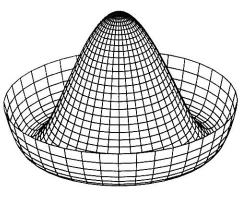
\includegraphics[width=0.3\linewidth]{Immagini - Capitolo 1/potenziale sombrero.png}
    \caption{andamento del potenziale a cappello messicano.}
    \label{fig: potenziale sombrero}
\end{figure}
In questo modo si trova la relazione tra il potenziale chimico, la costante di accoppiamento $g$ e la densità delle particelle con
\begin{equation}
    \mu = \frac{g\rho_0}{m} = g|\phi_0|^2.
\end{equation}
In conclusione, l'azione della teoria possiede una simmetria globale $U(1)$ poiché è invariante sotto l'aggiunta di un fattore costante nella fase della funzione d'onda. Lo stato fondamentale non possiede invece questa simmetria; infatti, la teoria prevede un continuo di vuoti degeneri e la funzione d'onda macroscopica per lo stato fondamentale
\begin{equation}
    \phi(\vr) \equiv \phi_0 = |\phi_0|e^{i\alpha},
\end{equation}
che ha una fase ben definita. Per un sistema relativisticamente invariante è abbastanza semplice dimostrare che esistono due tipi di eccitazioni legate al meccanismo della rottura spontanea di simmetria $U(1)$:
\begin{enumerate}
    \item un bosone a massa nulla, detto ``bosone di Goldstone'', associato a variazioni di fase della funzione d'onda;

    \item un bosone massivo, detto ``bosone di Anderson-Higgs, associato ad oscillazioni nel modulo $\phi$.
\end{enumerate}
Nel caso non relativistico è più complessa e conviene analizzare il problema in dettaglio.

\subsection{Pseudo-particelle di Bogoljubov}
Una classe importante dell'equazione di Gross-Pitaevskii \eqref{eq: equazione di Gross-Pitaevskii} corrisponde ad oscillazioni di piccola ampiezza dove le variazioni nello spazio e nel tempo di $\phi$, rispetto alla configurazione omogenea $\phi_0$, sono piccole
\begin{equation}
    \phi(\vr,t) = [\phi_0 + \theta(\vr,t)]e^{-i\mu t/\hbar},\quad |\phi_0|^2 = \frac{\mu}{g} = \frac{N_0}{V},
\end{equation}
dove ci si pone in $T = \SI{0}{\kelvin}$ e si trascura il fenomeno dello svuotamento quantistico. Si pone quindi
\begin{equation}
    \theta(\vr,t) = u_ke^{i(\vk\cdot\vr - \omega t)} + v_ke^{-i(\vk\cdot\vr - \omega t)},
\end{equation}
per cui 
\begin{equation}
    \begin{split}
        \phi(\vr,t) &= \phi_0e^{-i\mu t/\hbar} + [u_ke^{i[\vk\cdot\vr - (\omega + \mu/\hbar) t]} + v_ke^{-i(\vk\cdot\vr - (\omega - \mu/\hbar) t)}] \\
        &\equiv \phi_0e^{-i\mu t/\hbar} + \delta\phi,
    \end{split}
\end{equation}
che si sostituisce nell'equazione
\begin{equation}
\label{eq: equazione di schrodinger non lineare con Vext = 0 e V = g*delta}
    i\hbar\frac{\p}{\p t}\phi(\vr,t) + \frac{\hbar^2}{2m}\nabla^2\phi(\vr,t) = g|\phi(\vr,t)|^2\phi(\vr,t).
\end{equation}
Il contributo al primo ordine del membro di sinistra della \eqref{eq: equazione di schrodinger non lineare con Vext = 0 e V = g*delta} è
\begin{equation}
    \bigg[(\hbar\omega + \mu) - \frac{\hbar^2k^2}{2m}\bigg]u_ke^{i[\vk\cdot\vr - (\omega + \mu/\hbar)t]} + \bigg[(\mu - \hbar\omega) - \frac{\hbar^2k^2}{2m}\bigg]v_ke^{-i[\vk\cdot\vr - (\omega - \mu/\hbar)t]},
\end{equation}
dove si è trascurato il termine costante $\mu\phi_0$. Ponendo
\begin{equation}
    \phi(\vr,t) = \phi_0e^{-i\mu t/\hbar} + \delta\phi,\quad \phi^*(\vr,t) = \phi_0e^{i\mu t/\hbar} + \delta\phi^*,
\end{equation}
si ha
\begin{equation}
    \begin{split}
        g|\phi|^2\phi &= g(\phi_0e^{-i\mu t/\hbar} + \delta\phi)(\phi_0e^{i\mu t/\hbar} + \delta\phi^*)(\phi_0e^{-i\mu t/\hbar} + \delta\phi) \\
        &= g\phi_0^3e^{-i\mu t/\hbar} + 2g\phi_0^2\delta\phi + g\phi_0^2e^{-2i\mu t/\hbar}\delta\phi^* + O(\delta\phi^2);
    \end{split}
\end{equation}
trascurando il termine costante $g\phi_0^3e^{-i\mu t/\hbar}$, il termine di ordine $O(\delta\phi)$ è
\begin{equation}
    \begin{split}
        2\mu\delta\phi + \mu e^{-2i\mu t/\hbar}\delta\phi^* &= 2\mu(u_ke^{i[\vk\cdot\vr - (\omega + \mu/\hbar)t]} + v_ke^{-i[\vk\cdot\vr - (\omega - \mu/\hbar)t]}) \\
        &+ \mu e^{-2i\mu t/\hbar}(u_k^*e^{-i[\vk\cdot\vr - (\omega + \mu/\hbar)t]} + v_ke^{i[\vk\cdot\vr - (\omega - \mu/\hbar)t]}) \\
        &= \mu(2u_k + v_k^*)e^{i[\vk\cdot\vr - (\omega + \mu/\hbar)t]} \\
        &+ \mu(2v_k + u_k^*)e^{-i[\vk\cdot\vr - (\omega - \mu/\hbar)t]},
    \end{split}
\end{equation}
arrivando infine al sistema 
\begin{equation}
    \begin{cases}
        \bigg[(\hbar\omega + \mu) - \dfrac{\hbar^2k^2}{2m}\bigg]u_k = 2\mu u_k + \mu v_k^* \\[2ex]
        \bigg[(\mu - \hbar\omega) - \dfrac{\hbar^2k^2}{2m}\bigg]v_k^* = 2\mu v_k^* + \mu u_k
    \end{cases},
\end{equation}
il quale può essere riscritto in forma matriciale come
\begin{equation}
    \begin{pmatrix}
        \hbar\omega - \mu - \dfrac{\hbar^2k^2}{2m} & -\mu \\
        -\mu & -\mu - \hbar\omega - \dfrac{\hbar^2k^2}{2m}
    \end{pmatrix}
    \begin{pmatrix}
        u_k \\
        v_k^*
    \end{pmatrix}
    = 0.
\end{equation}
Questo sistema di equazioni risulta in soluzioni non banali se e solo se 
\begin{equation}
    \det{
    \begin{pmatrix}
        \hbar\omega - \mu - \dfrac{\hbar^2k^2}{2m} & -\mu \\
        -\mu & -\mu - \hbar\omega - \dfrac{\hbar^2k^2}{2m}
    \end{pmatrix}
    } = 0,
\end{equation}
da cui, tramite il calcolo esplicito
\begin{equation}
    \begin{split}
        \bigg(\hbar\omega - \mu - \frac{\hbar^2k^2}{2m}\bigg)\bigg(-\mu - \hbar\omega - \frac{\hbar^2k^2}{2m}\bigg) - \mu^2& = 0 \\
        \bigg[- \hbar^2\omega^2 + \bigg(\mu + \frac{\hbar^2k^2}{2m}\bigg)^2\bigg] - \mu^2 &= 0 \\
        \bigg(\mu + \frac{\hbar^2k^2}{2m}\bigg)^2 - \mu^2 &= \hbar^2\omega^2,
    \end{split}
\end{equation}
si può ricavare la relazione di dispersione di Bogoljubov
\begin{equation}
\label{eq: relazione di dispersione di Bogoljubov}
    \hbar\omega = \sqrt{\frac{\hbar^2k^2}{2m}\bigg(\frac{\hbar^2k^2}{2m} + 2\mu\bigg)}\quad\Longleftrightarrow\quad \epsilon(k) = \sqrt{\epsilon_0(k)[\epsilon_0(k) + 2\mu]}.
\end{equation}
\begin{obs}
    La relazione che si troverebbe al posto della \eqref{eq: relazione di dispersione di Bogoljubov} considerando il segno opposto quando si prende la radice ambo i membri corrisponde allo scambio $u_k\longleftrightarrow v_{-k}$: le due soluzioni rappresentano lo stesso tipo di oscillazione fisica.
\end{obs}
Considerando il limite in cui $k \to 0$ nella relazione trovata in \eqref{eq: relazione di dispersione di Bogoljubov} si ha 
\begin{equation}
    \hbar\omega \equiv \epsilon(k) \simeq \sqrt{\frac{\mu}{m}}\hbar k = v_1 q,\quad v_1 = \sqrt{\frac{\mu}{m}} = \sqrt{\frac{gn_0}{m}},
\end{equation} 
dove $v_1$ è la velocità del fonone. Quindi, la pseudo-particella di Bogoljubov corrispondente a questa legge di dispersione è un caso particolare di bosone di Goldstone per un condensato di particelle bosoniche debolmente interagenti. Invece, nel limite $k \to \infty$ si ha 
\begin{equation}
    \epsilon(k) = \epsilon_0(k)\sqrt{1 + \frac{2\mu}{\epsilon_0(k)}} \simeq \epsilon_0(k) + \mu,
\end{equation}
quindi la legge di dispersione tende asintoticamente, a meno della costante $\mu$, a quella di particella libera. In conclusione, l'interazione caratterizzata dal parametro $g > 0$ è responsabile della rottura spontanea di simmetria e della comparsa delle eccitazioni di Bogoljubov. Compare una ibridizzazione tra la curva di dispersione fononica e quella di particella libera, come mostrato in figura \ref{fig: e(q) regime fononico}.
\begin{figure}[h]
    \centering
    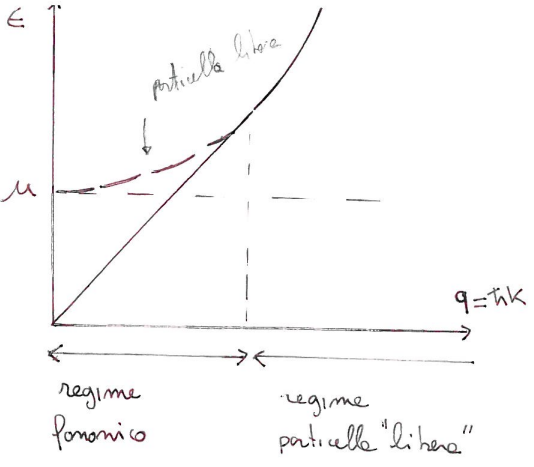
\includegraphics[width=0.4\linewidth]{Immagini - Capitolo 1/e(q) regime fononico.png}
    \caption{confronto tra le relazioni di dispersione nei regimi di particelle libera e fononico.}
    \label{fig: e(q) regime fononico}
\end{figure}
La funzione $\theta(\vr,t)$ può corrispondere ad oscillazioni di fase e modulo: non esiste una pseudo-particella di Anderson-Higgs distinta dal bosone di Goldstone nei condensati di Bose-Einstein.

\subsection{Solitone}
Si considerano ora delle soluzioni dell'equazione di Gross-Pitaevskii dipendente dal tempo che prendono il nome di  ``solitoni''. Nel caso repulsivo dove $g > 0$, queste soluzioni corrispondono a modulazioni della densità localizzate che si muovono nel condensato con velocità costante e preservando la loro forma nel tempo. Il profilo del solitone nella regione perturbata è caratterizzato da una diminuzione della densità $\rho_0$ rispetto al valore di bulk e si chiama ``solitone grigio''. L'esistenza di quest'ultimo è direttamente legata alla non linearità dell'equazione di Gross-Pitaevskii, il cui effetto compensa il termine quantistico di pressione associato all'energia cinetica. L'estensione spaziale del solitone è caratterizzata dalla lunghezza di ``healing'' $\xi$ definita come
\begin{equation}
\label{eq: lunghezza di healing}
    \xi = \frac{\hbar}{\sqrt{2m gn_0}},\quad n_0 = \frac{N_0}{V} \equiv \frac{N}{V}.
\end{equation}
Quindi, si ritorna all'equazione \eqref{eq: equazione di schrodinger non lineare con Vext = 0 e V = g*delta}, che si riporta qui per comodità 
\begin{equation}
    i\hbar\frac{\p}{\p t}\phi(\vr,t) = \bigg[-\frac{\hbar^2}{2m}\nabla^2 + g|\phi(\vr,t)|^2\bigg]\phi(\vr,t),
\end{equation}
e si considerano soluzioni che descrivono la propagazione di un fronte d'onda perpendicolare all'asse $z$, ossia della forma 
\begin{equation}
\label{eq: ansatz soluzione di solitone}
    \phi(\vr,t) = \sqrt{n_0}f(z,t)e^{-i\mu t/\hbar} \equiv \phi_s(\vr,t)e^{-i\mu t/\hbar},
\end{equation}
dove $f(z,t)$ è una funzione che dipende solo dalla coordinata cartesiana $z$. Quindi, sostituendo l'ansatz \eqref{eq: ansatz soluzione di solitone} nell'equazione \eqref{eq: equazione di schrodinger non lineare con Vext = 0 e V = g*delta} si ha
\begin{equation}
    \begin{split}
        i\hbar\frac{\p f(z,t)}{\p t} + \mu f(z,t) &= \bigg[-\frac{\hbar^2}{2m}\frac{\p^2}{\p z^2} + gn_0|f(z,t)|^2\bigg]f(z,t) \\
        i\hbar\frac{\p}{\p t}f(z,t) &= \bigg[-\frac{\hbar^2}{2m}\frac{\p^2}{\p z^2}f(z,t) + gn_0(|f(z,t)|^2 - 1)f(z,t)\bigg],
    \end{split}
\end{equation}
di cui si cercano soluzioni del tipo $f(z,t) \equiv f(z - vt)$. Con questa assunzione si trova
\begin{equation}
    -\frac{i\hbar v}{gn_0}\frac{df(z - vt)}{d(z - vt)} = -\frac{\hbar^2}{2mgn_0}\frac{d^2}{d(z - vt)^2}f(z - vt) + (|f(z - vt)|^2 - 1)f(z - vt),
\end{equation}
che definendo il parametro $\gamma$ tramite la lunghezza di healing, definita in equazione \eqref{eq: lunghezza di healing}, come
\begin{equation}
    \gamma \equiv \frac{z - vt}{\xi},
\end{equation}
diventa 
\begin{equation}
    -\frac{i\hbar v}{gn_0}\frac{\sqrt{2mgn_0}}{\hbar}\frac{df(\gamma)}{d\gamma} = -\frac{d^2f(\gamma)}{d\gamma^2} + (|f(\gamma)|^2 - 1)f(\gamma).
\end{equation}
Adesso, considerando che la velocità del suono $v_1$ nel condensato è pari a $v_1 = \sqrt{gn_0/m}$, si pone 
\begin{equation}
    \frac{v}{gn_0}\sqrt{2mgn_0} = \sqrt{2}v\sqrt{\frac{m}{gn_0}} = \sqrt{2}\frac{v}{v_1} \equiv 2U.
\end{equation}
Dunque, l'equazione che si deve risolvere è
\begin{equation}
\label{eq: equazione solitone in gamma}
    2iU\frac{df}{d\gamma} = \frac{d^2f}{d\gamma^2} + (1 - |f|^2)f,
\end{equation}
con l'obiettivo di trovare una soluzione localizzata che soddisfi le condizioni asintotiche
\begin{equation}
\label{eq: condizioni al bordo del solitone}
    \begin{cases}
        |f(\gamma)| \to 1 \\[2ex]
        \dfrac{df}{d\gamma} \to 0
    \end{cases},\quad \gamma \to \pm\infty.
\end{equation}
Per farlo, si moltiplica l'equazione appena trovata \eqref{eq: equazione solitone in gamma} per $f^*(\gamma)$ e se ne sottrae la complessa coniugata moltiplicata per $f$, ossia da 
\begin{equation}
    \begin{cases}
        2iUf^*\dfrac{df}{d\gamma} = f^*\dfrac{d^2f}{d\gamma^2} + (1 - |f^2|)|f^2| \\
        -2iUf\dfrac{df^*}{d\gamma} = f\dfrac{d^2f^*}{d\gamma^2} + (1 - |f^2|)|f^2|
    \end{cases}
\end{equation}
si ottiene
\begin{equation}
    2iU\bigg(f^*\frac{df}{d\gamma} + f\frac{df^*}{d\gamma}\bigg) = f^*\dfrac{d^2f}{f\gamma^2} - f\frac{d^2f^*}{d\gamma^2},
\end{equation}
la quale integrata in $d\gamma'$ sull'intervallo $\gamma' \in [\gamma,\infty]$ restituisce
\begin{equation}
\label{eq: equazione di continuità del solitone}
    2iU(1 - |f|^2) + f^*\frac{df}{d\gamma} - f\frac{df^*}{d\gamma} = 0,
\end{equation}
del tutto consistente con le condizioni al bordo imposte in \eqref{eq: condizioni al bordo del solitone}.
\begin{obs}
    Non è un caso che l'equazione \eqref{eq: equazione di continuità del solitone} abbia la forma di un'equazione di continuità, infatti il procedimento seguito per ottenerla è il medesimo usato in Meccanica quantistica per ottenere proprio l'equazione di continuità.
\end{obs}
Adesso, è possibile ottenere un'altra equazione a partire dalla \eqref{eq: equazione solitone in gamma} considerandone la parte immaginaria
\begin{equation}
    2U\frac{df_1}{d\gamma} = \frac{d^2f_2}{d\gamma^2} + (1 - f_1^2 - f_2^2)f_2,\quad f = f_1 + if_2,
\end{equation}
della quale si intende cercare soluzioni con $f_2 = \mathrm{costante}$, per cui l'equazione si riduce semplicemente a
\begin{equation}
\label{eq: equazione parte immaginaria solitone I}
    \frac{2U}{f_2}\frac{df_1}{d\gamma} = (1 - f_1^2 - f_2^2),
\end{equation}
sotto questa stessa assunzione l'equazione di continuità \eqref{eq: equazione di continuità del solitone} diventa 
\begin{equation}
    \begin{split}
        -2iU(1 - f_1^2 - f_2^2) &= (f_1 - if_2)\frac{d}{d\gamma}(f_1 + if_2) - (f_1 + if_2)\frac{d}{d\gamma}(f_1 - if_2) \\
        &= -2if_2\frac{df_1}{d\gamma},
    \end{split}
\end{equation}
ossia
\begin{equation}
\label{eq: equazione parte immaginaria solitone II}
    \frac{f_2}{U}\frac{df_1}{d\gamma} = (1 - f_1^2 - f_2^2).
\end{equation}
Le equazioni \eqref{eq: equazione parte immaginaria solitone I} e \eqref{eq: equazione parte immaginaria solitone II} coincidono se e solo se 
\begin{equation}
\label{eq: condizione su f2 per concidenza equazioni I e II}
    \frac{2U}{f_2} = \frac{f_2}{U}\quad\Longrightarrow\quad f_2 = \sqrt{2}U \equiv \frac{v}{v_1}.
\end{equation}
Quindi, sostituendo la condizione \eqref{eq: condizione su f2 per concidenza equazioni I e II} in una delle due equazioni si ha
\begin{equation}
    \sqrt{2}\dfrac{df_1}{d\gamma} = \bigg(1 - \frac{v^2}{v_1^2} - f_1^2\bigg),
\end{equation}
che può essere riscritta nella forma 
\begin{equation}
    \frac{d}{d\bigg(\gamma\sqrt{\dfrac{1 - v^2/v_1^2}{2}}\bigg)}\bigg(\frac{f_1}{\sqrt{1 - v^2/v_1^2}}\bigg) = \bigg[ 1 - \bigg(\frac{f_1}{\sqrt{1 - v^2/v_1^2}}\bigg)^2\bigg],
\end{equation}
così da poterla confrontare con la relazione generale
\begin{equation}
    \frac{d}{dx}\tanh{(x)} = 1 - \tanh^2{(x)}
\end{equation}
e ottenendo infine
\begin{equation}
\label{eq: soluzione f1 del solitone}
    f_1 = \sqrt{1 - \frac{v^2}{v_1^2}}\tanh{\bigg(\gamma\sqrt{\frac{1 - v^2/v_1^2}{2}}\bigg)}.
\end{equation}
Dunque, sostituendo l'espressione trovata per $f_1$ \eqref{eq: soluzione f1 del solitone} nell'ansatz originario \eqref{eq: ansatz soluzione di solitone} si ottiene la soluzione del solitone grigio
\begin{equation}
\label{eq: soluzione del solitone grigio}
    \phi_s(z - vt) = \sqrt{n_0}\bigg[\frac{iv}{v_1} + \sqrt{1 - \frac{v^2}{v_1^2}}\tanh{\bigg(\frac{z - vt}{\sqrt{2}\xi}\sqrt{1 - \frac{v^2}{v_1^2}}\bigg)}\bigg].
\end{equation}
Il profilo di densità $n(z - vt) = |\phi_s(z - vt)|^2$ ha la forma di una campana capovolta, come mostrato in figura \ref{fig: profilo densità solitone grigio}. Il minimo di questa funzione corrisponde alla condizione $z - vt = 0$, ossia a $\tanh{(0)} = 0$, che risulta nel valore
\begin{equation}
    n(0) = n_0\bigg|\frac{iv}{v_1}\bigg|^2 = n_0\frac{v^2}{v_1^2}. 
\end{equation}
\begin{obs}
    Per un solitone con velocità $v = 0$, ovvero per il quale il minimo del profilo di densità è $n(0) = 0$, si parla di ``dark soliton''.
\end{obs}
\begin{figure}[h]
    \centering
    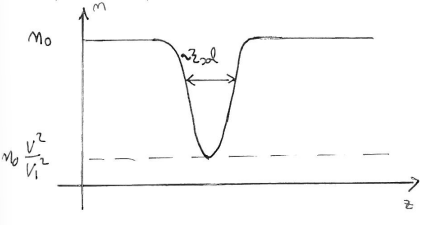
\includegraphics[width=0.5\linewidth]{Immagini - Capitolo 1/profilo densità solitone grigio.png}
    \caption{profilo di densità relativo alla soluzione del solitone grigio.}
    \label{fig: profilo densità solitone grigio}
\end{figure}
La fase della funzione d'onda subisce una variazione finita tra $z = -\infty$ e $z = \infty$, infatti partendo da
\begin{align}
    \phi_s(\infty) = i\sqrt{n_0}\bigg(\frac{v}{v_1} - i\sqrt{1 - \frac{v^2}{v_1}}\bigg), \\
    \phi_s(-\infty) = i\sqrt{n_0}\bigg(\frac{v}{v_1} + i\sqrt{1 - \frac{v^2}{v_1}}\bigg),
\end{align}
si può calcolare il rapporto 
\begin{equation}
    \frac{\phi_s(\infty)}{\phi_s(-\infty)} = e^{i\Delta\phi} = \bigg(\frac{v}{v_1} - i\sqrt{1 - \frac{v^2}{v_1^2}}\bigg)^2,
\end{equation}
da cui si trova che la differenza di fase è 
\begin{equation}
    \Delta\phi = 2\arccos{\bigg(\frac{v}{v_1}\bigg)}.
\end{equation}
\begin{obs}
    Per un ``dark soliton'' $\phi_s$ è reale e dispari, quindi la differenza di fase è pari a $\Delta\phi = \pi$, che corrisponde ad un ``difetto topologico'', ossia il fluido viene diviso a metà da uno strato di fluido in fase normale.
\end{obs}
La ``larghezza'' del solitone, mostrata in figura \ref{fig: profilo densità solitone grigio}, è legata alla lunghezza di healing tramite la relazione
\begin{equation}
    \xi_s = \frac{\xi}{\sqrt{1 - v^2/v_1^2}},
\end{equation}
la quale tende a divergere ad $\infty$ nel limite $v \to v_1$. Ora, è possibile calcolare l'energia del solitone per unità di superficie $\epsilon_s$ come
\begin{equation}
    \begin{split}
        \epsilon_s &= \int_\R dz\,\bigg[\frac{\hbar^2}{2m}\bigg|\frac{d\phi_s}{dz}\bigg|^2 + \bigg(\frac{g}{2}|\phi_s|^4 - gn_0|\phi_s|^2\bigg)\bigg] - \bigg(\frac{g}{2}|\phi_0|^4 - gn_0|\phi_0|^2\bigg). \\
        &= \int_\R dz\,\bigg[\frac{\hbar^2}{2m}\bigg|\frac{d\phi_s}{dz}\bigg|^2 + \frac{g}{2}(|\phi_s|^2 - n_0)^2\bigg],
    \end{split}
\end{equation}
dove il termine nella seconda parentesi tonda corrisponde all'energia dello stato imperturbato, per cui la differenza tra i due termini nelle tonde è la differenza tra le energie grancanoniche in presenza e in assenza del solitone; ad ogni modo, da questo, svolgendo l'integrale, si trova
\begin{equation}
    \epsilon_s = \frac{4}{3}\hbar v_1n_0\bigg( 1 - \frac{v^2}{v_1^2}\bigg)^{3/2}.
\end{equation}
Nel limite in cui $v \ll 1$, l'energia $\epsilon_s$ può essere espansa come
\begin{equation}
    \epsilon_s \simeq \frac{4}{3}\hbar v_1 n_0 - 2\hbar v_1 n_0 \frac{v^2}{v_1^2} = \frac{4}{3}\hbar v_1 n_0 + \frac{1}{2}\bigg(-\frac{4\hbar n_0}{v_1}\bigg)v^2,
\end{equation}
quindi il solitone si comporta come una particella di massa negativa
\begin{equation}
    m_s = -\frac{4\hbar n_0}{v_1},
\end{equation}
in accordo con il fatto che la modulazione di densità corrisponde ad una ``buca'' piuttosto che ad una ``particella''. Un fatto particolare, è che la velocità del solitone aumenta al decrescere dell'energia, questo vuole dire che in presenza di dissipazione dovuta alle collisioni con fononi a temperature $T > \SI{0}{\kelvin}$ il solitone accelera fino ad eventualmente scomparire quando $v \to v_1$. Quindi, il solitone è instabile per fluttuazioni nelle direzioni trasverse, per questo negli esperimenti con atomi freddi l'instabilità viene soppressa diminuendo le dimensioni trasversali tramite trappole magnetiche.

\section{Quantizzazione canonica}
Da un punto di vista formale, la Meccanica quantistica può essere interpretata come una deformazione della Meccanica classica, in cui le variabili classiche vengono sostituite da operatori che al posto di comparire nelle parentesi di Poisson compaiono nell'anticommutatore rispettivo. Quindi, date due variabili classiche $f$ e $g$ con la relazione
\begin{equation}
    \acomm{f}{g} = \sum_{i=1}^s\bigg(\frac{\p f}{\p q^i}\frac{\p g}{\p p_i} - \frac{\p f}{\p p_i}\frac{\p g}{\p q^i}\bigg),
\end{equation}
dove $s$ indica il numero di gradi di libertà del sistema, il passaggio alla trattazione quantistica consiste nel promuovere $f$ e $g$ al ruolo di operatori hermitiani $\hatf$ e $\hatg$, rispettivamente, e di definire una relazione di commutazione analoga alle parentesi di Poisson
\begin{equation}
     \acomm{f}{g} \xrightarrow{MQ} \frac{1}{i\hbar}\comm{\hatf}{\hatg} = \frac{1}{i\hbar} \sum_{i=1}^s\bigg(\frac{\p \hatf}{\p q^i}\frac{\p \hatg}{\p p_i} + \frac{\p \hatf}{\p p_i}\frac{\p \hatg}{\p q^i}\bigg),
\end{equation}
dove $\{q^i\}$ e $\{p_i\}$ sono le variabili canonicamente coniugate, ossia tali che
\begin{equation}
    \acomm{q^k}{p_j} = \sum_{i=1}^s\bigg(\frac{\p q_k}{\p q^i}\frac{\p p_j}{\p p_i} - \frac{\p q_k}{\p p_i}\frac{\p p_j}{\p q^i}\bigg) = \delta_{kj} \xrightarrow{MQ} \comm{\hatq_k}{\hatp_j} = i\hbar\delta_{kj}.
\end{equation}
L'evoluzione classica di una funzione $f$ è data da
\begin{equation}
    \frac{df}{dt} = \frac{\p f}{\p t} + \sum_{i=1}^s\bigg(\frac{\p f}{\p q^i}\frac{\p H}{\p p_i} - \frac{\p f}{\p p_i}\frac{\p H}{\p q^i}\bigg) = \frac{\p f}{\p t} + \acomm{f}{H} \xrightarrow{MQ} \frac{d\hatf}{dt} = \frac{\p\hatf}{\p t} + \comm{\hatf}{\hatH},
\end{equation}
dove $H(\vq,\vp)$ è l'hamiltoniana del sistema in Meccanica classica che soddisfa le equazioni di Hamilton
\begin{equation}
    \begin{cases}
        \dfrac{\p H}{\p p_i} = \dot{q}^i \\[2ex]
        \dfrac{\p H}{\p q^i} = -\dot{p}_i
    \end{cases},
\end{equation}
mentre $\hatH$ è l'operatore hamiltoniano in Meccanica quantistica. Si può poi introdurre la Lagrangiana del sistema come
\begin{equation}
    \dL(q_i,\dot{q}_i) = \sum_{i=1}^sp_i\dot{q}^i - H(\vq,\vp),
\end{equation}
da cui si definisce il momento canonicamente coniugato a $q^i$ come
\begin{equation}
    p_i = \frac{\p \dL}{\p \dot{q}^i}.
\end{equation}

\subsection{Oscillatore armonico come teoria di campo}
Si consideri l'hamiltoniana dell'oscillatore armonico 
\begin{equation}
\label{eq: hamiltoniana oscillatore armonico}
    H(\phi,\pi) = \frac{\pi(t)^2}{2m} + \frac{m\omega^2}{2}\phi(t)^2,
\end{equation}
dove $\phi$ e $\pi$ sono variabili canonicamente coniugate dalle relazioni
\begin{equation}
    \frac{\p H}{\p \pi} = \frac{\pi(t)}{m} = \dot{\phi}(t),\quad \frac{\p H}{\p \phi} = m\omega^2\phi(t) = -\dot{\pi}(t).
\end{equation}
In generale, esistono due modi per quantizzare il sistema dell'oscillatore armonico. Inizialmente, si può pensare di promuovere le variabili coniugate $\phi(t)$ e $\pi(t)$ al ruolo di operatori $\hatphi(t)$ e $\hatpi(t)$ con le relazioni di commutazione $\comm{\hatphi}{\hatpi} = i\hbar$ dove si passa
\begin{equation}
    \pi(t) \to \hatpi(t) = -i\hbar\frac{\p}{\p \phi},\quad \phi(t) \to \hatphi(t),
\end{equation}
in questo modo si arriva all'equazione di Schr\"odinger 
\begin{equation}
    \bigg(-\frac{\hbar^2}{2m}\frac{\p^2}{\p \phi^2} + \frac{m\omega}{2}\phi^2\bigg)\Psi(\phi,t) = i\hbar\frac{\p}{\p t}\Psi(\phi,t).
\end{equation}
Questo formalismo può essere utilizzato anche in una teoria di campo, ossia quando $\phi(\vr,t)$ dipende da un indice continuo $\vr$; tuttavia, è una tecnica non molto popolare a causa della perdita esplicita, nel caso di teorie invarianti relativistiche, della covarianza e delle difficoltà tecniche associate ad una trattazione rigorosa di equazioni alle derivate funzionali. In alternativa, si può dividere il campo $\phi(t)$ in due ``campi'' complessi
\begin{equation}
    \begin{cases}
        \phi(t) = \sqrt{\dfrac{\hbar}{2m\omega}}[a(t) + a^*(t)] \\[2ex]
        \pi(t) = \sqrt{\dfrac{m\omega\hbar}{2}}[a(t) - a^*(t)]
    \end{cases},
\end{equation}
da cui si ricavano le relazioni inverse
\begin{equation}
    \begin{cases}
        a(t) = \dfrac{i}{\sqrt{2\hbar m\omega}}\pi(t) + \sqrt{\dfrac{m\omega}{2\hbar}}\phi(t) \\
        a^*(t) = -\dfrac{i}{\sqrt{2\hbar m\omega}}\pi(t) + \sqrt{\dfrac{m\omega}{2\hbar}}\phi(t)
    \end{cases},
\end{equation}
che possono essere usate per riscrivere l'hamiltoniana nella \eqref{eq: hamiltoniana oscillatore armonico} come
\begin{equation}
    \begin{split}
        H &= \hbar\omega\bigg(-\dfrac{i}{\sqrt{2\hbar m\omega}}\pi(t) + \sqrt{\dfrac{m\omega}{2\hbar}}\phi(t)\bigg)\bigg(\dfrac{i}{\sqrt{2\hbar m\omega}}\pi(t) + \sqrt{\dfrac{m\omega}{2\hbar}}\phi(t)\bigg) \\
        &= \hbar\omega a^*(t)a(t).
    \end{split}
\end{equation}
Non è complesso vedere che il cambiamento di variabili $\{\phi,\pi\} \to i\hbar\{a,a^*\}$ corrisponde ad una trasformazione canonica
\begin{equation}
    \begin{split}
        i\hbar\acomm{a}{a^*} &= i\hbar\bigg(\frac{\p a}{\p \phi}\frac{\p a^*}{\p \pi} - \frac{\p a}{\p \pi}\frac{\p a^*}{\p \phi}\bigg) \\
        &= \bigg(-\dfrac{i}{\sqrt{2\hbar m\omega}}\sqrt{\dfrac{m\omega}{2\hbar}} -\dfrac{i}{\sqrt{2\hbar m\omega}}\sqrt{\dfrac{m\omega}{2\hbar}}\bigg) \\
        &= 1,
    \end{split}
\end{equation}
per quantizzare la teoria quindi si passa da
\begin{equation}
    i\hbar\acomm{a}{a^*} = 1 \xrightarrow{MQ} \comm{\hata}{\hataT} = 1,
\end{equation}
con la quale si può riscrivere l'operatore hamiltoniano come
\begin{equation}
    \hatH = \hbar\omega\bigg(\hataT\hata + \frac{1}{2}\bigg) \equiv \hbar\omega\bigg(\hatN + \frac{1}{2}\bigg),
\end{equation}
dove $\hatN := \hataT\hata$ è l'operatore numero che fornisce, tramite la sua equazione agli autovalori $\hatN\ket{N} = N\ket{N}$, il numero di quanti $N$. In Teoria dei campi l'idea è di identificare le particelle del sistema come gli autostati dell'hamiltoniana quantistica, ossia con le eccitazioni del campo ad energia definita, per cui gli operatori $\hata$ e $\hataT$ possono essere interpretati come gli operatori di distruzione di stati di particella con energia $\hbar\omega$ e di creazione di stati di particella con la medesima energia. Questi operatori agiscono su stati appartenenti ad uno spazio di Fock a numero finito di particelle; quindi, indicando con $\ko$ lo stato di vuoto, gli operatori si definiscono in modo che 
\begin{equation}
    \hata\ko = 0,\quad \hataT\ko = \ket{1},
\end{equation}
o su uno stato di $N$ particelle
\begin{equation}
    \hata\ket{N} = \sqrt{N}\ket{N - 1},\quad \hataT\ket{0} = \sqrt{N!}\ket{N}.
\end{equation}

\subsection{Quantizzazione dell'equazione di Gross-Pitaevskii}
L'equazione di Gross-Pitaevskii in seconda quantizzazione si ottiene, come nel caso dell'oscillatore armonico, individuando coppie di variabili classiche canonicamente coniugate e promuovendole al rango di operatori. La densità di lagrangiana di Gross-Pitaevskii è
\begin{equation}
    \dL_{GP} = i\hbar\phi^*(\vr,t)\frac{\p}{\p t}\phi(\vr,t) - \frac{\hbar^2}{2m}\nabla\phi^*(\vr,t)\nabla\phi(\vr,t) - \frac{g}{2}|\phi(\vr,t)|^4,
\end{equation}
quindi il momento coniugato a $\phi$ è 
\begin{equation}
    \pi(\vr,t) = \frac{\p \dL}{\p(\p_t\phi)} = i\hbar\phi^*(\vr,t).
\end{equation}
Promuovendo $\phi(\vr,t)$ e $\pi(\vr,t)$ ad operatori si definiscono le relazioni di commutazione a tempi uguali tra i due campi
\begin{equation}
\label{eq: relazioni di commutazione per campi bosonici}
    \begin{cases}
        \comm{\hatphi(\vr,t)}{\hatphid(\vr',t)} = \delta(\vr' - \vr) \\
        \comm{\hatphi(\vr,t)}{\hatphi(\vr',t)} = 0 \\ 
        \comm{\hatphid(\vr,t)}{\hatphid(\vr',t)} = 0
    \end{cases},
\end{equation}
da cui si capisce che i campi $\phi(\vr,t)$ e $\pi(\vr,t)$ seguono la statistica di Bose-Einstein. Se si definisce lo stato fondamentale $\kO$, allora il campo di creazione agisce su di esso come
\begin{equation}
    \hatphid(\vr)\kO = \ket{\vr},
\end{equation}
ovvero creando una particella con coordinate spaziali $\vr$; in modo analogo, lo stato a due particelle è dato da
\begin{equation}
    \frac{1}{\sqrt{2}}\hatphid(\vr_1)\hatphid(\vr_2)\kO = \ket{\vr_1,\vr_2} = \frac{1}{\sqrt{2}}\hatphid(\vr_2)\hatphid(\vr_1)\kO = \ket{\vr_2,\vr_1},
\end{equation}
che risulta essere simmetrico per lo scambio delle particelle dato che la statistica è quella bosonica. In generale, lo stato ad $N$ particella è completamente simmetrico sotto lo scambio di qualsiasi coppia di particelle ed è dato da
\begin{equation}
    \ket{\vr_1,\dots,\vr_N} = \frac{1}{\sqrt{N!}}\hatphid(\vr_1)\cdots\hatphid(\vr_N)\kO.
\end{equation}
L'hamiltoniana di Gross-Pitaevskii in seconda quantizzazione è
\begin{equation}
    \hatH_{GP} = \int d^3r\bigg[\hatphid(\vr)\bigg(-\frac{\hbar^2}{2m}\nabla^2\bigg)\hatphi(\vr) + \frac{g}{2}\hatphid(\vr)^2\hatphi(\vr)^2\bigg],
\end{equation}
la quale agisce sullo stato fondamentale annichilandolo, ossia $\hatH_{GP}\kO = 0$. Un generico stato fisico $\ket{\Phi(t)}$ deve essere una soluzione dell'equazione di Schr\"odinger 
\begin{equation}
    i\hbar\frac{\p}{\p t}\ket{\Phi(t)} = \hatH_{GP}\ket{\Phi(t)}.
\end{equation}
Si calcola ora il commutatore dell'hamiltoniana $\hatH_{GP}$ con il campo $\hatphid(\vr)$
\begin{equation}
    \begin{split}
        \comm{\hatH_{GP}}{\hatphid(\vr)} &= \int d^3r_1\bigg[\hatphid(\vr_1)\bigg(-\frac{\hbar^2}{2m}\nabla^2_{\vr_1}\bigg)\hatphi(\vr_1) + \frac{g}{2}\hatphid(\vr)^2\hatphi(\vr)^2,\hatphid(\vr)\bigg] \\
        &= \int d^3r_1\bigg\{-\frac{\hbar^2}{2m}\nabla^2_{\vr_1}\hatphid(\vr_1)\comm{\hatphi(\vr_1)}{\hatphid(\vr)} \\
        &+ g\hatphid(\vr_1)^2\hatphi(\vr_1)\comm{\hatphi(\vr_1)}{\hatphid(\vr)}\bigg\} \\
        &= -\frac{\hbar^2}{2m}\nabla^2\hatphid(\vr) + g\hatphid(\vr)^2\hatphi(\vr),
    \end{split}
\end{equation}
dove si sono usate nell'ultimo passaggio le relazioni di commutazioni definite nella \eqref{eq: relazioni di commutazione per campi bosonici}; quindi il commutatore cercato vale
\begin{equation}
\label{eq: commutatore H_GP e phiT}
    \comm{\hatH_{GP}}{\hatphid(\vr)} = \bigg[-\frac{\hbar^2}{2m}\nabla^2 + g\hatphid(\vr)\hatphi(\vr)\bigg]\hatphid(\vr),
\end{equation}
con il quale si può scrivere l'equazione di Gross-Pitaevskii per il campo $\hatphid$ come
\begin{equation}
\label{eq: equazione di Gross-Pitaevskii per campo phiT}
    i\hbar\frac{\p}{\p t}\hatphid(\vr) = -\comm{\hatH_{GP}}{\hatphid(\vr)}.
\end{equation}

\subsubsection{Stato ad una particella}
Ci consideri ora lo stato ad una particella $\ket{\vr} = \hatphid(\vr)\kO$ e se ne calcoli la norma
\begin{equation}
    \begin{split}
        \mybraket{\vr_1}{\vr} = \mybrakett{\Omega}{\hatphi(\vr_1)\hatphid(\vr)}{\Omega} &= \mybrakett{\Omega}{\comm{\hatphi(\vr_1)}{\hatphid(\vr)}}{\Omega} \\
        &= \mybrakett{\Omega}{\delta(\vr_1 - \vr)}{\Omega} \\
        &= \delta(\vr_1 - \vr),
    \end{split}
\end{equation}
mentre la relazione di completezza è
\begin{equation}
    \int d^3r\,\ket{\vr}\bra{\vr} = \MI.
\end{equation}
Uno stato fisico $\ket{\Phi(t)}$ ad una particella può essere quindi rappresentato utilizzando la base $\{\vr\}$ come
\begin{equation}
    \ket{\Phi(t)} = \int d^3r\,\ket{\vr}\mybraket{\vr}{\Phi(t)} = \int d^3r\,\Phi(\vr,t)\ket{\vr},
\end{equation}
dove $\Phi(\vr,t)$ è la funzione che determina la particolare sovrapposizione di autostati di posizione $\ket{\vr}$ che compongono $\ket{\Phi(t)}$. Si vuole ora dimostrare che $\Phi(\vr,t)$ soddisfa l'equazione di Schr\"odinger della particella libera 
\begin{equation}
\label{eq: equazione di schrodinger della particella libera}
    i\hbar\frac{\p}{\p t}\Phi(\vr,t) = -\frac{\hbar^2}{2m}\nabla^2\Phi(\vr,t);
\end{equation}
per farlo si calcola esplicitamente
\begin{equation}
    \begin{split}
        i\hbar\frac{\p}{\p t}\ket{\Phi(t)} &= \int d^3r\bigg(i\hbar\frac{\p}{\p t}\Phi(\vr,t)\bigg)\ket{\vr} \\
        &= \hatH_{GP}\ket{\Phi(\vr,t)} \\
        &= \int d^3r\,\Phi(\vr,t)\hatH_{GP}\hatphid(\vr)\kO \\
        &= \int d^3r\,\Phi(\vr,t)\comm{\hatH_{GP}}{\hatphid(\vr)}\kO \\
        &= \int d^3r\,\Phi(\vr,t)\bigg[-\frac{\hbar^2}{2m}\nabla^2\hatphid(\vr) + g\hatphid(\vr)^2\hatphi(\vr)\bigg]\kO \\
        &= \int d^3r\bigg(-\frac{\hbar^2}{2m}\nabla^2\bigg)\Phi(\vr,t)\hatphid(\vr)\kO \\
        &= \int d^3r\bigg(-\frac{\hbar^2}{2m}\nabla^2\Phi(\vr,t)\bigg)\ket{r},
    \end{split}
\end{equation}
dove nel secondo passaggio si è usata l'equazione \eqref{eq: equazione di Gross-Pitaevskii per campo phiT}, nel quarto si è usata la relazione \eqref{eq: commutatore H_GP e phiT} e infine nel quinto si è integrato due volte per parti in modo ``da spostare'' l'operatore $\nabla^2$; quindi, confrontando gli integrandi nel primo e nell'ultimo passaggio si trova direttamente quanto volevasi dimostrare
\begin{equation}
    i\hbar\frac{\p}{\p t}\Phi(\vr,t) = -\frac{\hbar^2}{2m}\nabla^2\Phi(\vr,t).
\end{equation}

\subsubsection{Stato a due particelle}
Si consideri ora lo stato a due particelle 
\begin{equation}
    \ket{r_1,r_2} = \frac{1}{\sqrt{2}}\hatphid(\vr_1)\hatphid(\vr_2)\kO
\end{equation}
e se ne calcoli la norma 
\begin{equation}
    \begin{split}
        \mybraket{r_1,r_2}{r_1',r_2'} &= \frac{1}{2}\mybrakett{\Omega}{\hatphi(\vr_1)\hatphi(\vr_2)\hatphid(\vr_1')\hatphid(\vr_2')}{\Omega} \\
        &= \frac{1}{2}\mybrakett{\Omega}{\hatphi(\vr_2)\{\comm{\hatphi(\vr_1)}{\hatphid(\vr_1')} + \hatphid(\vr_1')\hatphi(\vr_1)\}\hatphid(\vr_2')}{\Omega} \\
        &= \frac{1}{2}\mybrakett{\Omega}{\hatphi(\vr_2)[\delta(\vr_1 - \vr_1') + \hatphid(\vr_1')\hatphi(\vr_1)]\hatphid(\vr_2')}{\Omega} \\
        &= \frac{1}{2}\mybrakett{\Omega}{\hatphi(\vr_2)\delta(\vr_1 - \vr_1')\hatphid(\vr_2')}{\Omega} \\
        &+ \frac{1}{2}\mybrakett{\Omega}{\hatphi(\vr_2)\hatphid(\vr_1')\comm{\hatphi(\vr_1)}{\hatphid(\vr_2')}}{\Omega} \\
        &= \frac{1}{2}\delta(\vr_1 - \vr_1')\delta(\vr_2 - \vr_2') + \frac{1}{2}\delta(\vr_2 - \vr_1')\delta(\vr_1 - \vr_2').
    \end{split}
\end{equation}
Questa norma suggerisce che si sta studiando un sistema a due particelle identiche, infatti la norma è diversa da zero se e solo se
\begin{equation}
    \begin{cases}
        r_1 = r_1' \\
        r_2 = r_2'
    \end{cases}
    \quad \vee \quad\quad
    \begin{cases}
        r_1 = r_2' \\
        r_2 = r_1'
    \end{cases}.
\end{equation}
Un generico stato $\ket{\Phi(t)}$ a due particelle può quindi essere sviluppato sulla base $\ket{r_1,r_2}$ come
\begin{equation}
    \begin{split}
        \ket{\Phi(t)} &= \int d^3r_1\,d^3r_2\, \Phi(\vr_1,\vr_2,t)\ket{\vr_1,\vr_2} \\
        &= \frac{1}{\sqrt{2}}\int d^3r_1\,d^3r_2\,\Phi(\vr_1,\vr_2,t)\hatphid(\vr_1)\hatphid(\vr_2)\kO,
    \end{split}
\end{equation}
dove, poiché $\comm{\hatphid(\vr_1)}{\hatphid(\vr_2)} = 0$, l'integrale su $r_1$ e $r_2$ è simmetrico sotto lo scambio $(\vr_1 \longleftrightarrow \vr_2)$ quindi $\Phi(\vr_1,\vr_2,t) = \Phi(\vr_2,\vr_1,t)$ e si ha
\begin{equation}
\label{eq: equazione di schrodinger a due particelle}
    i\hbar\frac{\p}{\p t}\ket{\Phi(t)} = \int d^3r_1\,d^3r_2\,\bigg[i\hbar\frac{\p}{\p t}\Phi(\vr_1,\vr_2,t)\bigg]\ket{\vr_1,\vr_2}.
\end{equation}
A destra dell'equazione di Schr\"odinger \eqref{eq: equazione di schrodinger a due particelle} si ha
\begin{equation}
    \begin{split}
        \hatH_{GP}\ket{\Phi(t)} &= \frac{1}{\sqrt{2}}\int d^3r_1\,d^3r_2\,\Phi(\vr_1,\vr_2,t)\hatH_{GP}\hatphid(\vr_1)\hatphid(\vr_2)\kO \\
        &= \frac{1}{\sqrt{2}}\int d^3r_1\,d^3r_2\,\Phi(\vr_1,\vr_2,t) \\ &\times(\comm{\hatH_{GP}}{\hatphid(\vr_1)} + \hatphid(\vr_1)\hatH_{GP})\hatphid(\vr_2)\kO \\
        &= \frac{1}{\sqrt{2}}\int d^3r_1\,d^3r_2\bigg[-\frac{\hbar^2}{2m}\nabla^2_{\vr_1}\hatphid(\vr_1) + g\hatphid(\vr_1)^2\hatphi(\vr_1)\bigg] \\
        &\times\Phi(\vr_1,\vr_2,t)\hatphid(\vr_2)\kO + \frac{1}{2}\int d^3r_1\,d^3r_2\,\Phi(\vr_1,\vr_2,t)\hatphid(\vr_1) \\
        &\times\comm{\hatH_{GP}}{\hatphid(\vr_2)}\kO,
    \end{split}
\end{equation}
dove nell'ultimo passaggio si è usato che $\hatH_{GP}\kO = 0$, ora integrando per parti il primo termine si ha
\begin{equation}
    \begin{split}
        \hatH_{GP}\ket{\Phi(t)} &= \frac{1}{\sqrt{2}}\int d^3r_1\,d^3r_2\bigg[\hatphid(\vr_1)\bigg(-\frac{\hbar^2}{2m}\nabla^2_{\vr_1}\bigg) + g\hatphid(\vr_1)^2\hatphi(\vr_1)\bigg] \\
        &\times\Phi(\vr_1,\vr_2,t)\hatphid(\vr_2)\kO + \frac{1}{\sqrt{2}}\int d^3r_1\,d^3r_2\,\hatphid(\vr_1)\Phi(\vr_1,\vr_2,t) \\
        &\times\bigg[-\frac{\hbar^2}{2m}\nabla^2_{\vr_2}\hatphid(\vr_2) + g\hatphid(\vr_2)^2\hatphi(\vr_2)\bigg]\kO \\
        &= \frac{1}{\sqrt{2}}\int d^3r_1\,d^3r_2\bigg[-\frac{\hbar^2}{2m}\nabla^2_{\vr_1}\Phi(\vr_1,\vr_2,t)\bigg]\hatphid(\vr_1)\hatphid(\vr_2)\kO \\
        &+ \frac{1}{\sqrt{2}}\int d^3r_1\,d^3r_2\, g\hatphid(\vr_1)^2\delta(\vr_1 - \vr_2)\Phi(\vr_1,\vr_2,t)\kO \\
        &+ \frac{1}{\sqrt{2}}\int d^3r_1\,d^3r_2\,\bigg[-\frac{\hbar^2}{2m}\nabla^2_{\vr_2}\Phi(\vr_1,\vr_2,t)\bigg]\hatphid(\vr_1)\hatphid(\vr_2)\kO \\
        &= \int d^3r_1\,d^3r_2\bigg[-\frac{\hbar^2}{2m}\nabla^2_{\vr_1} -\frac{\hbar^2}{2m}\nabla^2_{\vr_2}\bigg]\Phi(\vr_1,\vr_2,t)\ket{\vr_1,\vr_2} \\
        &+ \int d^3r_1\,d^3r_2\,g\delta(\vr_1 - \vr_2)\Phi(\vr_1,\vr_2,t)\ket{\vr_1,\vr_2},
    \end{split}
\end{equation}
dove si è usata la proprietà $\hatphid(\vr_1)^2\delta(\vr_1 - \vr_2) = \hatphid(\vr_1)\hatphid(\vr_2)\delta(\vr_1 - \vr_2)$ e integrato per parti nel secondo passaggio. Finalmente, si arriva a 
\begin{multline}
    \int d^3r_1\,d^3r_2\,\bigg[i\hbar\frac{\p}{\p t}\Phi(\vr_1,\vr_2,t)\bigg]\ket{\vr_1,\vr_2} = \\ = \int d^3r_1\,d^3r_2\bigg[-\frac{\hbar^2}{2m}\nabla^2_{\vr_1} -\frac{\hbar^2}{2m}\nabla^2_{\vr_2} + g\delta(\vr_1 - \vr_2)\bigg]\Phi(\vr_1,\vr_2,t)\ket{\vr_1,\vr_2},
\end{multline}
la quale porta all'equazione di Schr\"odinger a due corpi con un potenziale a delta di Dirac
\begin{equation}
    i\hbar\frac{\p}{\p t}\Phi(\vr_1,\vr_2,t) = \bigg[-\frac{\hbar^2}{2m}\nabla^2_{\vr_1} -\frac{\hbar^2}{2m}\nabla^2_{\vr_2} + g\delta(\vr_1 - \vr_2)\bigg]\Phi(\vr_1,\vr_2,t).
\end{equation}
Nel caso di un sistema ad $N$ particelle, lo stato è dato da
\begin{equation}
    \ket{\Phi(t)} = \frac{1}{\sqrt{N!}}\int d^3r_1\cdots d^3r_N\,\Phi(\vr_1,\dots,\vr_N,t)\hatphid(\vr_1)\cdots\hatphid(\vr_N)\kO.
\end{equation}
\begin{obs}
    Un risultato simile si sarebbe potuto ottenere anche con un potenziale generico $V(\vr_1 - \vr_2)$.
\end{obs}
In conclusione, si è dimostrato che l'hamiltoniana in seconda quantizzazione $\hatH_{GP}$, quando ristretta ad un sottospazio con $N$ fissato, è equivalente ad un'equazione di Schr\"odinger a molti corpi con un interazione descritta dalla delta di Dirac e della statistica bosonica. Per sistemi non relativistici la ``seconda quantizzazione'' è solo un modo più conveniente per formulare la Meccanica quantistica a molti corpi. In Meccanica quantistica relativistica il numero di particelle non è in generale conservato e il formalismo della seconda quantizzazione è l'unico utilizzabile.
\begin{center}
    \begin{tikzpicture}[
        box/.style = {rectangle, draw, rounded corners=2mm, thin, minimum width=2.5cm, minimum height=1.4cm, align=center}, node distance=2.5cm]
        \node[box] (a) {Equazione di Schr\"odinger \\ a $N$ corpi con potenziale \\ a delta di Dirac};
        \node[box, right=of a] (b) {Equazione di Gross-Pitaevskii \\ in seconda quantizzazione};
        \node[box, below=of $(a)!0.5!(b)$] (c){Equazione di Gross-Pitaevskii ``classica''};
          
        \draw[<-] (a) -- node[above, align=center]{sottospazio \\ con $N$ fisso } (b);
        \draw[<-] (b) -- node[right=8pt, align=left]{ quantizzazione canonica \\ del campo di G-P} (c);
        \draw[<-] (c) -- node[left=8pt, align=right]{$N \gg 1$ campo medio \\ di Hartree-Fock} (a);
    \end{tikzpicture}
\end{center}

\subsubsection{Operatore numero di particelle}
Il numero di particelle in un determinato stato $\ket{\Phi(t)}$ è un autovalore dell'operatore
\begin{equation}
    \hatN = \int dr\,\hatphid(\vr)\hatphi(\vr),\quad \hatN\kO = 0.
\end{equation}
Calcolando i commutatori
\begin{align}
    \comm{\hatN}{\hatphi(\vr)} = \int dr_1\,\comm{\hatphid(\vr_1)\hatphi(\vr_1)}{\hatphi(\vr)} = -\int dr_1\delta(\vr_1 - \vr)\hatphi(\vr_1) = -\hatphi(\vr), \\
    \comm{\hatN}{\hatphid(\vr)} = \int dr_1\,\comm{\hatphid(\vr_1)\hatphi(\vr_1)}{\hatphid(\vr)} = \int dr_1\delta(\vr_1 - \vr)\hatphid(\vr_1) = \hatphid(\vr),
\end{align}
si possono riscrivere come
\begin{equation}
    \begin{cases}
        \hatN\hatphid(\vr) = \hatphid(\vr)(\hatN + 1) \\
        \hatN\hatphi(\vr) = \hatphi(\vr)(\hatN - 1)
    \end{cases};
\end{equation}
quindi per uno stato ad $N$ particelle si ha
\begin{equation}
    \begin{split}
        \hatN\ket{\vr_1,\dots,\vr_N} &= \frac{1}{\sqrt{N!}}\hatN\hatphid(\vr_1)\cdots\hatphid(\vr_N)\kO \\
        &= \frac{1}{\sqrt{N!}}\hatphid(\vr_1)\cdots\hatphid(\vr_N)(\hatN + N)\kO \\
        &= N\ket{\vr_1,\dots,\vr_N}.
    \end{split}
\end{equation}

\section{Spazio dei momenti}
Risulta probabilmente più intuitivo considerare gli operatori di creazione e distruzione nello spazio dei momenti dato che l'hamiltoniana è diagonale in tale spazio in assenza di un potenziale di interazione. Si supponga che il sistema sia contenuto in un volume $V = L^3$ con condizioni periodiche al bordo, in tal caso si può sviluppare il campo $\hatphi(\vr)$ in serie di Fourier 
\begin{equation}
    \hatphi(\vr) = \frac{1}{\sqrt{V}}\nsum_k\hata_ke^{i\vk\cdot\vr},\quad \vk = \frac{2\pi\hbar}{L}(n_x,n_y,n_z),\quad n_x,n_y,n_z \in \Z,
\end{equation}
per cui la trasformazione inversa è
\begin{equation}
    \hata_k = \frac{1}{\sqrt{V}}\int d^3r\,\hatphi(\vr)e^{-i\vk\cdot\vr},
\end{equation}
con la quale si può calcolare il commutatore
\begin{equation}
    \begin{split}
        \comm{\hata_k}{\hataT_q} &= \frac{1}{V}\int d^3r\,d^3r_1\comm{\hatphi(\vr)e^{-i\vk\cdot\vr}}{\hatphid(\vr)e^{i\vq\cdot\vr_1}} \\
        &= \frac{1}{V}\int d^3r\,d^3r_1\,\delta(\vr - \vr_1)e^{-i\vk\cdot\vr}e^{i\vq\cdot\vr_1} \\
        &= \frac{1}{V}\int d^3r\,e^{i(\vk - \vq)\vr} \\
        &= \delta_{k,q},
    \end{split}
\end{equation}
che corrisponde proprio alla relazione di commutazione canonica tra $\hata$ e $\hataT$ dell'oscillatore armonico; naturalmente, valgono anche le relazioni $\comm{\hata_k}{\hata_q} = \comm{\hataT_k}{\hataT_q} = 0$. Si riscrive quindi l'hamiltoniana $\hatH_{GP}$ nello spazio dei momenti come
\begin{equation}
    \begin{split}
        \hatH_{GP} &= \int d^3r\bigg[\hatphid(\vr)\bigg(-\frac{\hbar^2}{2m}\nabla^2\bigg)\hatphi(\vr) + \frac{g}{2}\hatphid(\vr)^2\hatphi(\vr)^2\bigg] \\
        &\equiv \int d^3r\,(\hatT_{GP} + \hatV_{GP}),
    \end{split}
\end{equation}
dove il termine cinetico è
\begin{equation}
    \begin{split}
        \hatT_{GP} &= \int d^3r\,\hatphid(\vr)\bigg(-\frac{\hbar^2}{2m}\nabla^2\bigg)\hatphi(\vr) \\
        &= \frac{1}{V}\int d^3r\,\sum_{k,q}\hataT_qe^{-iqr}\bigg(-\frac{\hbar^2}{2m}\nabla^2\bigg)\hata_ke^{i\vk\cdot\vr} \\
        &= \sum_{k,q}\hataT_q\hata_k\bigg(\frac{\hbar^2k^2}{2m}\bigg)\frac{1}{V}\int d^3r\,e^{-i(\vq - \vk)\cdot r} \\
        &= \sum_{k,q}\hataT_q\hata_k\bigg(\frac{\hbar^2k^2}{2m}\bigg)\delta_{k,q} \\
        &= \nsum_{k}\frac{\hbar^2k^2}{2m}\hataT_k\hata_k \\
        &\equiv \nsum_{k}\frac{\hbar^2k^2}{2m}\hatN_k,
    \end{split}
\end{equation}
mentre quello di interazione è
\begin{equation}
    \begin{split}
        \hatV_{GP} &= \frac{g}{2}\int d^3r\,\hatphid(\vr)\hatphid(\vr)\hatphi(\vr)\hatphi(\vr) \\
        &= \frac{g}{2V^2}\sum_{\substack{k1,k_2 \\ q_1,q_2}}\int d^3r\,\hataT_{q_2}\hataT_{q_1}\hata_{k_1}\hata_{k_2}e^{i(q_1 + q_2 - k_1 - k_1)r} \\
        &= \frac{g}{2V}\sum_{\substack{k1,k_2 \\ q_1,q_2}}\hataT_{q_2}\hataT_{q_1}\hata_{k_1}\hata_{k_2}\delta_{k_1 + k_2, q_1 + q_2}.
    \end{split}
\end{equation}
Quindi, l'interpretazione dell'hamiltoninana nello spazio dei momenti 
\begin{equation}
\label{eq: hamiltoniana nello spazio dei momenti}
    \hatH_{GP} = \nsum_k\frac{\hbar^2k^2}{2m}\hataT_k\hata_k + \frac{g}{2V}\sum_{\substack{k1,k_2 \\ q_1,q_2}}\hataT_{q_2}\hataT_{q_1}\hata_{k_1}\hata_{k_2}\delta_{k_1 + k_2, q_1 + q_2}
\end{equation}
consiste nelle seguenti osservazioni:
\begin{enumerate}
    \item il termine cinetico $\hatT_{GP}$ è interpretato come l'operatore che conta il numero di particelle con momento $\vk$ e che associa ad ognuna di esse un'energia $\hbar^2k^2/2m$ ;
    \item il termine di potenziale $\hatV_{GP}$ causa la scattering annichilendo due particelle con impulso $\vk_1$ e $\vk_2$ e creandone altre due con impulso $\vq_1$ e $\vq_2$, conservando sempre il momento totale con $\vk_1 + \vk_2 = \vq_1 + \vq_2$.
\end{enumerate}
Usando la conservazione del quadrimpulso codificata dalla $\delta_{k_1 + k_2, q_1 + q_2}$ si può riscrivere il termine di interazione nella \eqref{eq: hamiltoniana nello spazio dei momenti} come
\begin{equation}
    \hatV_{GP} = \frac{g}{2V}\sum_{\substack{k1,k_2 \\ q}}\hataT_{k_2 + q}\hataT_{k_1 - q}\hata_{k_1}\hata_{k_2}.
\end{equation}
\begin{obs}
    Se ci fosse un termine che non conserva il numero di particelle, ad esempio $\hataT\hataT\hataT\hata\hata$, non sarebbe possibile stabilire l'equivalenza con l'equazione di Schr\"odinger a molti corpi. In questi casi la trattazione tramite la Teoria dei campi è l'unica possibile.
\end{obs}

\section{Stati coerenti}
Dalla Meccanica quantistica è noto che lo stato fondamentale dell'oscillatore armonico minimizza il principio di indeterminazione di Heisenberg 
\begin{equation}
    \vmedio{(\Delta\hatphi)^2}_0\vmedio{(\Delta\hatpi)^2}_0 = \frac{\hbar^2}{4},
\end{equation}
dove $\Delta\hatphi = \hatphi - \vmedio{\hatphi}_0 = \hatphi$ e $\Delta\hatpi = \hatpi - \vmedio{\hatpi}_0 = \hatpi$. Non è complesso dimostrare che invece lo stato ad $N$ particelle non minimizza il principio di indeterminazione, infatti
\begin{align}
    \mybrakett{N}{(\hata + \hataT)(\hata + \hataT)}{N} &= \mybrakett{N}{\hata\hataT + \hataT\hata}{N} \notag \\
    &= \mybrakett{N}{2\hataT\hata + \comm{\hata}{\hataT}}{N} \\
    &= 2N + 1, \notag \\
    \mybrakett{N}{(\hata + \hataT)(\hata + \hataT)}{N} &= -(2N + 1),
\end{align}
poiché gli operatori si possono esprimere come
\begin{equation}
    \begin{cases}
        \hata - \hataT = i\sqrt{\dfrac{2}{m\omega\hbar}}\hatpi \\[2ex]
        \hata + \hataT = \sqrt{\dfrac{2m\omega}{\hbar}}\hatphi
    \end{cases}
\end{equation}
si ottiene
\begin{equation}
    \vmedio{(\Delta\hatphi)^2}_N\vmedio{(\Delta\hatpi)^2}_N = \frac{\hbar^2}{4}(2N + 1)^2.
\end{equation}
Questo dimostra che la parte destra dell'uguaglianza dipende da $N$ ed è minima per $N = 0$; quindi, il principio di indeterminazione non è minimizzato se si considerano valori medi sullo stato con numero di particelle fissato. Per il vuoto funziona perché $\hata\ko = 0\ko$, cioè $\ko$ è autostato di $\hata$. Se si considera ora un autostato generico di $\hata$ con autovalore $\alpha \in \C$ definito da
\begin{equation}
    \begin{cases}
        \hata\ket{\alpha} = \alpha\ket{\alpha} \\
        \bra{\alpha}\hataT = \alpha^*\ket{\alpha}
    \end{cases}
    ,\quad \mybraket{\alpha}{\alpha} = 1,
\end{equation}
si hanno $\mybrakett{\alpha}{(\hata + \hataT)}{\alpha} = \alpha + \alpha^*$ e $\mybrakett{\alpha}{(\hata - \hataT)}{\alpha} = \alpha - \alpha^*$ con i quali si calcola
\begin{align}
    \begin{split}
        \mybrakett{\alpha}{(\hata + \hataT)(\hata + \hataT)}{\alpha} &= \mybrakett{\alpha}{\hata^2 + (\hataT)^2 + \hata\hataT + \hataT\hata}{\alpha} \\
        &= \alpha^2 + (\alpha^*)^2 + 2\alpha^*\alpha + 1 \\
        &= (\alpha + \alpha^*)^2 + 1
    \end{split} \\
    \begin{split}
        \mybrakett{\alpha}{(\hata - \hataT)(\hata - \hataT)}{\alpha} &= \mybrakett{\alpha}{\hata^2 + (\hataT)^2 - \hata\hataT - \hataT\hata}{\alpha} \\
        &= \alpha^2 + (\alpha^*)^2 - 2\alpha^*\alpha - 1 \\
        &= (\alpha - \alpha^*)^2 - 1.
    \end{split}
\end{align}
Quindi, si calcolano
\begin{align}
    \begin{split}
        \vmedio{(\Delta\hatphi)^2}_\alpha = \vmedio{\hatphi^2}_\alpha - \vmedio{\hatphi}_\alpha^2 &= \frac{\hbar}{2m\omega}[(\alpha + \alpha^*)^2 + 1 - (\alpha + \alpha^*)^2] \\
        &= \frac{\hbar}{2m\omega},
    \end{split} \\
    \begin{split}
        \vmedio{(\Delta\hatpi)^2}_\alpha = \vmedio{\hatpi^2}_\alpha - \vmedio{\hatpi}_\alpha^2 &= -\frac{m\omega}{2\hbar}[(\alpha - \alpha^*)^2 - 1 - (\alpha - \alpha^*)^2] \\
        &= \frac{m\omega}{2\hbar}.
    \end{split}
\end{align}
Dunque, si ottiene la relazione di indeterminazione
\begin{equation}
\label{eq: principio di indeterminazione}
    \vmedio{(\Delta\hatphi)^2}_\alpha\vmedio{(\Delta\hatpi)^2}_\alpha = \frac{\hbar^2}{4}
\end{equation}
e lo stato $\ket{\alpha}$ minimizza il principio di indeterminazione per ogni $\alpha \in \C$. Il fatto che gli stati coerenti minimizzano il principio di indeterminazione è molto importante perché se si interpreta $\hata$ come il campo $\hatphi$ dell'equazione di Gross-Pitaesvkii, il valore di aspettazione di $\hata$ deve essere diverso da zero, come lo deve essere quello di $\hatphi$, così da poter ottenere $\mybrakett{\alpha}{\hata}{\alpha} = \alpha$.
\begin{obs}
    In questo caso si è posto $t = 0$, ma il risultato finale vale per ogni $t$, in accordo con l'idea che la coerenza viene conservata nel tempo.
\end{obs}
Lo stato coerente $\ket{\alpha}$ può essere rappresentato come somma infinita, con particolari coefficienti, nella base dello spazio di Fock come
\begin{equation}
    \ket{\alpha} = e^{-|\alpha|^2/2}\sum_{N=0}^\infty\frac{\alpha^N}{\sqrt{N!}}\ket{N},
\end{equation}
sul quale può agire l'operatore $\hata$ nel modo seguente
\begin{equation}
    \begin{split}
        \hata\ket{\alpha} &= e^{-|\alpha|^2/2}\sum_{N=1}^\infty\frac{\alpha^N\sqrt{N}}{\sqrt{(N - 1)!\sqrt{N}}}\ket{N - 1} \\
        &= \alpha e^{-|\alpha|^2/2}\sum_{N=1}^\infty\frac{\alpha^{N - 1}}{\sqrt{(N - 1)!}}\ket{N - 1} \\
        &= \alpha\ket{\alpha},
    \end{split}
\end{equation}
o alternativamente come
\begin{equation}
    \begin{split}
        \ket{\alpha} = e^{-(|\alpha|^2/2) + \alpha\hataT}\ko &=  e^{\alpha\hataT - \alpha^*\hata}\ko \\
        &= e^{-|\alpha|^2/2}\sum_{N=0}^\infty\frac{\alpha^N(\hataT)^N}{N!}\ko \\
        &= e^{-|\alpha|^2/2}\sum_{N=0}^\infty\frac{\alpha^N}{\sqrt{N!}}\ket{N},
    \end{split}
\end{equation}
dove nel primo passaggio si è usata la relazione di Baker-Campbell-Hausdorff
\begin{equation}
    e^{\hatA + \hatB} = e^{-\comm{\hatA}{\hatB}/2}e^{\hatA} e^{\hatB},
\end{equation}
che vale solamente se il commutatore dei due operatori commuta con i medesimi operatori singolarmente
\begin{equation}
    \comm{\comm{\hatA}{\hatB}}{\hatA} = \comm{\comm{\hatA}{\hatB}}{\hatB} = 0,
\end{equation}
dove $\hatA$ e $\hatB$ non commutano necessariamente tra di loro. Inoltre, l'evoluzione temporale di $\hata$ è dettata da
\begin{equation}
    \hata(t) = \hata e^{-i\omega t} = \hata e^{-i(\p E/\p N)t/\hbar} \equiv \hata e^{-i\mu t/\hbar},
\end{equation}
dove quindi è il potenziale chimico $\mu$, e non l'energia $E$, a determinare l'evoluzione temporale dello stato coerente. L'operatore 
\begin{equation}
    \hatD(\alpha) := e^{\alpha\hataT - \alpha^*\hata},
\end{equation}
tale che $\hatD(\alpha)\ko = \ket{\alpha}$, è detto operatore di Glauber. Questo operatore è unitario dato che $\hat\hatD(\alpha)\hatD^\dg(\alpha) = \MI$, inoltre usando il lemma di Hadamard
\begin{equation}
    e^{\hatA} e^{\hatB} = \hatB + \comm{\hatA}{\hatB} + \frac{1}{2!}\comm{\hatA}{\comm{\hatA}{\hatB}} + \cdots,
\end{equation}
con $\hatA = \alpha\hataT - \alpha^*\hata$ e $\hatB = \hata$ in modo che $\comm{\hatA}{\hatB} = \alpha$, si trova che
\begin{equation}
    \begin{cases}
        \hatD(\alpha)\hata\hatD(\alpha) = \hata - \alpha \\
        \hatD(\alpha)\hataT\hatD^\dg(\alpha) = \hataT - \alpha^*
    \end{cases};
\end{equation}
quindi, l'operatore di Glauber trasla il campo $\hata$ di un fattore $\alpha$ costante. Due stati coerenti $\ket{\alpha}$ e $\ket{\beta}$ non sono ortogonali, ossia $\mybraket{\alpha}{\beta} \neq 0$ per $\alpha \neq \beta$; infatti lo si può vedere calcolando
\begin{align}
    \begin{split}
        \mybraket{\alpha}{\beta} &= e^{-|\alpha|^2/2}e^{-|\beta|^2/2}\nsum_N\nsum_{N'}\frac{(\alpha^*)^N(\beta)^{N'}}{\sqrt{N!}\sqrt{N'!}}\mybraket{N}{N'} \\
        &= e^{-|\alpha|^2/2 -|\beta|^2/2 - \alpha^*\beta},
    \end{split} \\
    |\mybraket{\alpha}{\beta}|^2 &= e^{-|\alpha|^2 -|\beta|^2 + \alpha^*\beta + \alpha\beta^*} = e^{-|\alpha - \beta|^2},
\end{align}
ma per $|\alpha| = |\beta| \to \infty$, allora $|\mybraket{\alpha}{\beta}|^2 \to 0$. Adesso, introducendo la fase con $\alpha = |\alpha|e^{i\theta}$, si ha che lo stato è
\begin{equation}
    \ket{\alpha} = e^{|\alpha|^2/2}\nsum_N\frac{|\alpha|^N}{\sqrt{N!}}e^{i\theta N}\ket{N},\quad \ket{N} \propto \int_0^{2\pi}\frac{d\theta}{2\pi}e^{-i\theta N}\ket{\alpha(\theta)}.
\end{equation}
Quindi, le variabili $N$ e $\theta$ sono canonicamente coniugate:
\begin{enumerate}
    \item per $\ket{N}$, $N$ è fissato e $\theta$ è massimalmente indeterminato;
    \item per $\ket{\alpha}$, $\theta$ è fissato a meno di una fase di $2\pi$ ed $N$ è indeterminato.
\end{enumerate}
\begin{ex}
    Si considera un oscillatore armonico con un potenziale $V(\phi)$ quadratico centrato in $\phi = 0$; lo stato fondamentale è una gaussiana, con zero nodi e gli stati eccitati sono caratterizzati da un nodo al centro e antisimmetrici. Ponendo $m = \hbar = \omega = 1$, si ha
    \begin{equation}
        \mybraket{\phi}{0} = e^{\phi^2/2},\quad \hatH_0 = \frac{1}{2}\bigg(-\frac{d^2}{d\phi^2} + \phi^2\bigg),
    \end{equation}
    e si considera un'altra hamiltoniana associata ad un altro sistema traslato rispetto al primo
    \begin{equation}
        \hatH_\alpha = \frac{1}{2}\bigg[-\frac{d^2}{d\phi^2} + (\phi - \sqrt{2}\alpha)^2\bigg].
    \end{equation}
    Gli autovalori e le autofunzioni del sistema traslato sono collegate in modo semplice rispetto a quello originale, ma non sono identici; si scrive quindi la proiezione di $\alpha$ su $\phi$, dove $\ket{\alpha}$ è lo stato di vuoto traslato, ottenendo
    \begin{equation}
        \begin{split}
            \mybraket{\phi}{\alpha} = \exp{\bigg[-\frac{(\phi - \sqrt{2}\alpha)^2}{2}\bigg]} &= e^{-\alpha^2/2}\exp{\bigg[-\frac{(\phi - \sqrt{2}\alpha)^2}{2} + \frac{\alpha^2}{2}\bigg]} \\
            &= e^{-\alpha^2/2}\sum_{n=0}^\infty\frac{\alpha^n}{n!}\frac{H_n(\phi)}{(\sqrt{2})^n}e^{-\phi^2/2} \\
            &= e^{\alpha^2/2}\sum_{n=0}^\infty\frac{\alpha^n}{\sqrt{n!}}\ket{n}.
        \end{split}
    \end{equation}
    Compare quindi un termine gaussiano che caratterizza le soluzioni dell'oscillatore armonico, incluso il termine legato agli stati eccitati, dove $H_n(\phi)$ sono i polinomi di Hermite i cui zeri corrispondono a quelli della funzione d'onda; alla fine del calcolo ricompare lo stato coerente. 
\end{ex}
Gli stati che minimizzano il principio di indeterminazione tra $\hatphi$ e $\hatpi$ in equazione \eqref{eq: principio di indeterminazione} sono stati coerenti
\begin{equation}
    \ket{\alpha} = e^{|\alpha|^2/2}\sum_{N=0}^\infty\frac{\alpha^N}{\sqrt{N!}}\ket{N},
\end{equation}
ossia stati a numero di particelle non determinato, ovvero con $\vmedio{(\Delta\hatN)^2}_\alpha \neq 0$. In Meccanica statistica, nella descrizione grancanonica il numero di particelle del sistema non è fissato, ma lo è $\vmedio{\hatN}_\alpha$, dato da
\begin{equation}
    \vmedio{\Delta\hatN}_\alpha = \mybrakett{\alpha}{\hataT\hata}{\alpha} = |\alpha|^2,
\end{equation}
mentre il valore medio di $\hatN^2$ è dato da
\begin{equation}
    \begin{split}
        \vmedio{(\Delta\hatN)^2}_\alpha = \mybrakett{\alpha}{\hataT\hata\hataT\hata}{\alpha} &= \mybrakett{\alpha}{\hataT(\hataT\hata + 1)\hata}{\alpha} \\
        &= |\alpha|^4 + |\alpha|^2 \\
        &= \vmedio{\hatN}_\alpha^2 + \vmedio{\hatN}_\alpha.
    \end{split} 
\end{equation}
Poiché $\ket{\alpha}$ non è uno stato a numero ben definito di particelle, la deviazione standard è diversa da zero. Tuttavia, ci si potrebbe chiedere perché se nello stato $\ket{\alpha}$ la fase di $\hata$ è completamente determinata, la deviazione non è infinita. Il motivo è che l'operatore associato alla fase $\theta$, $\hatheta$, non è hermitiano, ossia non è un'osservabile. Infatti, si può scrivere
\begin{equation}
    \begin{cases}
        \hata = \sqrt{\hatN}e^{i\hatheta} \equiv \sqrt{\hatN}\hatU \\
        \hataT = \sqrt{\hatN}e^{-i\hatheta} \equiv \sqrt{\hatN}\hatU^\dg
    \end{cases},
\end{equation}
dove l'azione di $\hatU$ porta alle relazioni
\begin{equation}
    \begin{cases}
        \hata\ket{N} = \sqrt{N}\ket{N - 1} \\
        \hataT\ket{N} = \sqrt{N + 1}\ket{N + 1}
    \end{cases}.
\end{equation}
Adesso si deve capire se $\hatU$ è unitario, per farlo si considerano 
\begin{equation}
    \begin{cases}
        \hatU\ket{N} = \ket{N - 1} \\
        \hatU\ko = 0
    \end{cases},
\end{equation}
da cui si deduce che $\hatU^\dg\ket{N} = \ket{N + 1}$, quindi si trova che
\begin{equation}
    \begin{cases}
        \mybrakett{m}{\hatU\hatU^\dg}{n} = \delta_{m,n} \\
        \mybrakett{m}{\hatU^\dg\hatU}{n} = \delta_{m,n}
    \end{cases},\quad m,n > 0,
\end{equation}
tuttavia, per $ m = n = 0$ si ha anche che
\begin{equation}
    \mybrakett{0}{\hatU^\dg\hatU}{0} = 0 \quad\Longrightarrow\quad \hatU\hatU^\dg = 1 \neq \hatU^\dg\hatU,
\end{equation}
ossia che $\hatheta$ non commuta con $\hatheta^\dg$, dunque non è un'osservabile. Tuttavia, il problema diventa trascurabile se $\vmedio{\hatN}_\alpha \gg 1$ per cui le propabalità che lo stato coerente sia quello di vuoto o di $n$ particelle sono rispettivamente
\begin{equation}
    |\mybraket{0}{\alpha}|^2 = e^{-\vmedio{\hatN}_\alpha} \to 0,\quad |\mybraket{n}{\alpha}|^2 = e^{-\vmedio{\hatN}_\alpha}\frac{\vmedio{\hatN}^n_\alpha}{n!} \to 0,
\end{equation}
dove nella prima relazione sopravvive solo l'esponenziale nella definizione di $\alpha$, mentre nella seconda è calcolato su un numero finito di particelle. Per $n \ll \vmedio{\hatN}_\alpha$, si ha $\hatheta \simeq \hatheta^\dg$, quindi in questo caso si ha
\begin{equation}
    \sigma_{\hatN}\sigma_{\hatheta} \ge \frac{1}{2}\quad\Longrightarrow\quad \sigma_{\hatheta} \simeq \frac{1}{\sqrt{\vmedio{\Delta\hatN}_\alpha}}
\end{equation}
e la fase diventa localizzata per $\vmedio{\hatN} \to \infty$ ed osservabile, quindi trattabile come una variabile classica. Inoltre, per piccole fluttuazioni di densità si ha
\begin{equation}
    \sigma_{|\alpha|} \simeq \frac{\p|\alpha|}{\p\vmedio{\hatN}}\sigma_{\hatN} \simeq \frac{1}{2} = o(1) \ll \sqrt{\vmedio{\hatN}}.
\end{equation}
Dunque, nel limite in cui $N \to \infty$, è possibile sostituire gli operatori $\hata$ e $\hataT$ con i corrispondenti valori classici
\begin{equation}
    \hata = \sqrt{\hatN}e^{i\hatheta} \to a = \sqrt{\vmedio{\hatN}}e^{i\theta},\quad \hataT = \sqrt{\hatN}e^{-i\hatheta} \to a^* = \sqrt{\vmedio{\hatN}}e^{-i\theta}.
\end{equation}
Riassumendo brevemente quanto detto:
\begin{enumerate}
    \item gli stati coerenti permettono la localizzazione della fase e di trattare l'operatore $\hata$ come una quantità classica quando $\vmedio{\hatN} \gg 1$ passando ad $a = \sqrt{\vmedio{\hatN}}e^{i\theta}$;
    \item il valore di aspettazione del campo $\hata$ è nullo sul vuoto $\ko$, ma è diverso da zero sul vuoto coerente $\ket{\alpha}$ dove avviene una rottura spontanea di simmetria tramite $\mybrakett{\alpha}{\hata}{\alpha} = \alpha = \sqrt{N_0}e^{i\theta}$;
    \item l'operatore che crea lo stato coerente agendo su $\ko$ è l'operatore $\hatD(\alpha)$ di traslazione di campo;
    \item gli stati coerenti emergono in modo naturale quando si cerca di descrivere lo stato di minima energia nella fase dove la simmetria è rotta da $\vmedio{\hatphi(\vr,t)} \neq 0$, usando come base gli stati dello spazio di Fock del sistema a simmetria non rotta, dove $\vmedio{\hatphi(\vr,t)} = 0$.
\end{enumerate}
\begin{figure}[h]
    \centering
    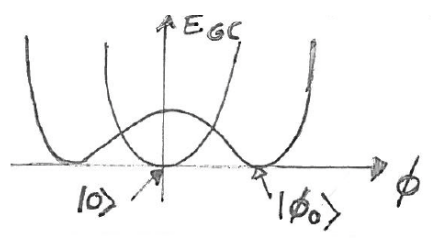
\includegraphics[width=0.4\linewidth]{Immagini - Capitolo 1/stati coerenti.png}
    \caption{stato di vuoto e stato coerente come stato di minima energia nella fase a simmetria rotta.}
    \label{fig: stati coerenti}
\end{figure}

\section{Approssimazione di Bogoljubov}
Si comincia separando la parte corrispondente allo stato fondamentale $\ko$ contenente gli operatori $\hata_0$ e $\hataT_0$ da quella relativa agli stati con $\vk \neq \vo$ considerandone solamente i termini quadratici in $\hata_k$, quindi l'hamiltoninana di partenza è
\begin{equation}
\label{eq: hamiltoniana G-P per approx. Bogoljubov}
    \begin{split}
        \hatH_{GP} &= \nsum_k\frac{\hbar^2k^2}{2m}\hataT_k\hata_k + \frac{g}{2V}\hataT_0\hataT_0\hata_0\hata_0 \\
        &+ \frac{g}{2V}\sum_{\vk \neq \vo}(4\hataT_0\hataT_k\hata_0\hata_k + \hataT_k\hataT_{-k}\hata_0\hata_0 + \hataT_0\hataT_0\hata_{-k}\hata_k) + o[(\hata_k)^3].
    \end{split}
\end{equation}
Infatti, nel termine $\sum_{k_1,k_2,q}\hataT_{k_2 + q}\hataT_{k_1 - q}\hata_{k_2}\hata_{k_1}$ ci sono sei termini che dipendono da due operatori $\hata_0$:
\begin{enumerate}
    \item $\hataT_q\hataT_{-q}\hata_0\hata_0$ per $(\vk_1 = \vo, \vk_2 = \vo)$;
    \item $\hataT_{k_2}\hataT_0\hata_{k_2}\hata_0$ per $(\vk_1 = \vo, \vk_1 - \vq = \vo)$;
    \item $\hataT_0\hataT_{k_2}\hata_{k_2}\hata_0$ per $(\vk_1 = \vo, \vk_2 + \vq = \vo)$;
    \item $\hataT_{k_1}\hataT_0\hata_0\hata_{k_1}$ per $(\vk_2 = \vo, \vk_1 - \vq = \vo)$;
    \item $\hataT_0\hataT_{k_1}\hata_0\hata_{k_1}$ per $(\vk_2 = \vo, \vk_2 + \vq = \vo)$;
    \item $\hataT_0\hataT_0\hata_{-k_1}\hata_{k_1}$ per $(\vk_1 - \vq = \vo, \vk_2 + \vq = \vo)$.
\end{enumerate}
Di questi sei termini $\hataT_q\hataT_{-q}\hata_0\hata_0$ e $\hataT_0\hataT_0\hata_{-k_1}\hata_{k_1}$ sono distinti, mentre gli altri quattro sono equivalenti a meno di rinominare le variabili, per cui 
\begin{equation}
    \hataT_{k_2}\hataT_0\hata_{k_2}\hata_0 + \hataT_0\hataT_{k_2}\hata_{k_2}\hata_0 + \hataT_{k_1}\hataT_0\hata_0\hata_{k_1} + \hataT_0\hataT_{k_1}\hata_0\hata_{k_1} = 4\hataT_0\hataT_k\hata_0\hata_k.
\end{equation}
Questi tre termini possono poi essere rappresentati graficamente come mostrato in figura \ref{fig: scattering 1, 2, 3}, interpretandoli come: lo scattering elastico tra una particella con $\vk \neq \vo$ e una del condensato; due particelle con impulso $\vk$ e $-\vk$ che escono dal condensato; due particelle con impulso $\vk$ e $-\vk$ che entrano nel condensato. In particolare, gli ultimi due processi non comportano una violazione della conservazione dell'energia in quanto le onde piane, ossia le particelle libere, non sono autofunzioni di $\hatH_{GP}$.
\begin{figure}[h]
    \centering
    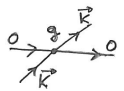
\includegraphics[width=0.2\linewidth]{Immagini - Capitolo 1/scattering 1.png}
    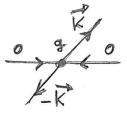
\includegraphics[width=0.2\linewidth]{Immagini - Capitolo 1/scattering 2.png}
    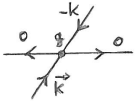
\includegraphics[width=0.2\linewidth]{Immagini - Capitolo 1/scattering 3.png}
    \caption{i termini di scattering distinti dell'hamiltoniana $\hatH_{GP}$ sono: (i) $\hataT_0\hataT_k\hata_0\hata_k$; (ii) $\hataT_k\hataT_{-k}\hata_0\hata_0$; (iii) $\hataT_0\hataT_0\hata_{-k}\hata_k$.}
    \label{fig: scattering 1, 2, 3}
\end{figure}

Si supponga ora che lo stato con $\vk = \vo$, su cui agiscono gli operatori $\hataT_0$ e $\hata_0$, sia uno stato coerente occupato in media dalla quasi totalità delle particelle, ossia $\hatN_0 \simeq \hatN$; per cui da
\begin{equation}
    \hatN = \hataT_0\hata_0 + \sum_{\vk \neq \vo}\hataT_k\hata_k = \hatN_0 + \sum_{\vk \neq \vo}\hataT_k\hata_k,
\end{equation}
si scrive il numero di particelle nello stato fondamentale in funzione di $\hatN$ invertendo la relazione
\begin{equation}
    \hatN_0 = \hatN - \sum_{\vk \neq \vo}\hataT_k\hata_k,
\end{equation}
considerando il termine $\sum_{\vk \neq \vo}\hataT_k\hata_k$ come una correzione al primo ordine dell'ordine zero $\hatN$. Si può allora scrivere il secondo termine dell'hamiltoniana \eqref{eq: hamiltoniana G-P per approx. Bogoljubov} come
\begin{equation}
    \begin{split}
        \frac{g}{2V}(\hataT_0\hataT_0\hata_0\hata_0) &= \frac{g}{2V}(\hatN^2 - 2\hatN\sum_{\vk \neq \vo}\hataT_k\hata_k) + \cdots \\
        &\simeq \frac{g}{2V}(N^2 - 2N\sum_{\vk \neq \vo}\hataT_k\hata_k),
    \end{split}
\end{equation}
dove si è sostituito a $\hatN$ il suo valore medio $\vmedio{\hatN} \equiv N$; l'hamiltoniana in questione quindi diventa l'hamiltoniana di Bogoljubov
\begin{equation}
\label{eq: hamiltoniana di Bogoljubov}
    \begin{split}
        \hatH_{GP} &\simeq \frac{gN^2}{2V} + \sum_{\vk \neq \vo}\frac{\hbar^2k^2}{2m}\hataT_k\hata_k - \frac{2gN}{2V}\sum_{\vk \neq \vo}\hataT_k\hata_k \\
        &+ \frac{g}{2V}\sum_{\vk \neq \vo}(4\hataT_0\hataT_k\hata_0\hata_k + \hataT_k\hataT_{-k}\hata_0\hata_0 + \hataT_0\hataT_0\hata_{-k}\hata_k) \\
        &= \frac{gN^2}{2V} + \sum_{\vk \neq \vo}\bigg(\frac{\hbar^2k^2}{2m} + \frac{2gN}{V}\bigg)\hataT_k\hata_k + \frac{gN}{2V}\sum_{\vk \neq \vo}(\hataT_k\hataT_{-k} + \hata_{-k}\hata_k) \\
        &\equiv \hatH_B
    \end{split}
\end{equation}
L'hamiltoniana $\hatH_B$ trovata può essere diagonalizzata attraverso la trasformazione di Bogoljubov.

\subsection{Trasformazione di Bogoljubov}
Prima di diagonalizzare direttamente $\hatH_B$, si considera un'hamiltoniana generica della forma
\begin{equation}
\label{eq: hamiltoniana generica h}
    \hath = \bar{\epsilon}(\hataT_1\hata_1 + \hataT_2\hata_2) + \lambda(\hataT_1\hataT_2 + \hata_2\hata_1),
\end{equation}
dove il secondo termine corrisponde ad un termine di interazione in quanto ``mescola'' gli operatori con indici diversi. Ad ogni modo, l'hamiltoniana $\hath$ può essere diagonalizzata utilizzando la trasformazione di Bogoljubov nel modo seguente. Si introducono due coppie di operatori di distruzione e creazione $(\hatd_1, \hatdT_1)$ e $(\hatd_2, \hatdT_2)$, legati agli operatori $(\hata_1, \hataT_1)$ e $(\hata_2, \hataT_2)$ attraverso la trasformazione canonica $\comm{\hatd_1}{\hatdT_1} = \comm{\hatd_2}{\hatdT_2} = 1$; si definisce la trasformazione di Bogoljubov
\begin{equation}
    \begin{cases}
        \hata_1 = u\hatd_1 + v\hatdT_2 \\
        \hataT_1 = u\hatdT_1 + v\hatd_2 \\
    \end{cases},\quad 
    \begin{cases}
        \hata_2 = u\hatd_2 + v\hatdT_1 \\
        \hataT_2 = u\hatdT_2 + v\hatd_1 \\
    \end{cases},\quad u,v \in \R,
\end{equation}
che infatti soddisfano le relazioni di commutazione
\begin{align}
    \begin{split}
        \comm{\hata_1}{\hataT_1} = \comm{u\hatd_1 + v\hatdT_2}{u\hatdT_1 + v\hatd_2} &= u\comm{\hatd_1}{u\hatdT_1 + v\hatd_2} + v\comm{\hatdT_2}{u\hatdT_1 + v\hatd_2} \\
        &= u^2\comm{\hatd_1}{\hatdT_1} + v^2\comm{\hatdT_2}{\hatd_2} \\
        &= u^2 - v^2 \\
        &= 1,
    \end{split} \\
    \begin{split}
        \comm{\hata_2}{\hataT_2} = \comm{u\hatd_2 + v\hatdT_1}{u\hatdT_2 + v\hatd_1} &= u\comm{\hatd_2}{u\hatdT_2 + v\hatd_1} + v\comm{\hatdT_1}{u\hatdT_2 + v\hatd_1} \\
        &= u^2\comm{\hatd_2}{\hatdT_2} + v^2\comm{\hatdT_1}{\hatd_1} \\
        &= u^2 - v^2 \\
        &= 1.
    \end{split}
\end{align}
Da queste ultime due relazioni si può pensare di parametrizzare i coefficienti $u$ e $v$ come $u = \cosh{\alpha}$ e $v = \sinh{\alpha}$, dove $\alpha$ deve essere fissato in modo da diagolinazzare $\hath$, così da poter usare anche le proprietà trigonometriche $u^2 + v^2 = \cosh{(2\alpha)}$ e $2uv = \sinh{(2\alpha)}$. Adesso, si riscrive $\hath$ in forma matriciale
\begin{equation}
\label{eq: hamiltoniana generica h in forma matriciale}
    \hath = \frac{1}{2}
    \begin{pmatrix}
        \hataT_1 & \hata_2 & \hataT_2 & \hata_1
    \end{pmatrix}
    \begin{pmatrix}
        \bar{\epsilon} & \lambda & 0 & 0 \\
        \lambda & \bar{\epsilon} & 0 & 0 \\
        0 & 0 & \bar{\epsilon} & \lambda \\
        0 & 0 & \lambda & \bar{\epsilon}
    \end{pmatrix}
    \begin{pmatrix}
        \hata_1 \\
        \hataT_2 \\
        \hata_2 \\
        \hataT_1
    \end{pmatrix} - \bar{\epsilon}
\end{equation}
\begin{obs}
    Si può verificare che effettivamente la riscrittura \eqref{eq: hamiltoniana generica h in forma matriciale} dell'hamiltoniana \eqref{eq: hamiltoniana generica h} considerando che la parte diagonale è
    \begin{equation}
        \begin{split}
            \frac{1}{2}
            \begin{pmatrix}
            \hataT_1 & \hata_2 & \hataT_2 & \hata_1
        \end{pmatrix}
        \begin{pmatrix}
            \hata_1 \\
            \hataT_2 \\
            \hata_2 \\
            \hataT_1
        \end{pmatrix} &= \frac{1}{2}\bar{\epsilon}(\hataT_1\hata_1 + \hata_2\hataT_2 + \hataT_2\hata_2 + \hata_1\hataT_1) \\
        &= \bar{\epsilon}(\hataT_1\hata_1 + \hataT_2\hata_2) + \bar{\epsilon},
        \end{split}
    \end{equation}
    mentre la parte non diagonale restituisce per il primo blocco
    \begin{equation}
        \frac{1}{2}
            \begin{pmatrix}
                \hataT_1 & \hata_2
            \end{pmatrix}
            \begin{pmatrix}
                0 & \lambda \\
                \lambda & 0
            \end{pmatrix}
            \begin{pmatrix}
                \hata_1 \\
                \hataT_2
            \end{pmatrix} = \frac{\lambda}{2}(\hataT_1\hataT_2 + \hata_2\hata_1),
    \end{equation}
    e per il secondo blocco un risultato analogo semplicemente scambiando gli indici $1$ e $2$; mettendo tutto insieme si ottiene proprio l'espressione \eqref{eq: hamiltoniana generica h}.
\end{obs}
Si parte dal primo blocco della matrice diagonale
\begin{equation}
    \begin{pmatrix}
        \hataT_1 & \hata_2
    \end{pmatrix}
    \begin{pmatrix}
        \bar{\epsilon} & \lambda \\
        \lambda & \bar{\epsilon}
    \end{pmatrix}
    \begin{pmatrix}
        \hata_1 \\
        \hataT_2
    \end{pmatrix}
\end{equation}
da cui, sostituendo la trasformazione di Bogoljubov definita dalle espressioni
\begin{equation}
    \begin{pmatrix}
        \hata_1 \\
        \hataT_2
    \end{pmatrix} = 
    \begin{pmatrix}
        u & v \\
        v & u
    \end{pmatrix}
    \begin{pmatrix}
        \hatd_1 \\
        \hatdT_2
    \end{pmatrix}, \quad 
    \begin{pmatrix}
        \hataT_1 & \hata_2
    \end{pmatrix} = 
    \begin{pmatrix}
        \hatdT_1 & \hatd_2
    \end{pmatrix}
    \begin{pmatrix}
        u & v \\
        v & u
    \end{pmatrix},
\end{equation}
si trova che
\begin{multline}
    \begin{pmatrix}
        \hatdT_1 & \hatd_2
    \end{pmatrix}
    \begin{pmatrix}
        u & v \\
        v & u
    \end{pmatrix}
    \begin{pmatrix}
        \bar{\epsilon}u + \lambda v & \bar{\epsilon}v + \lambda u \\
        \bar{\epsilon}v + \lambda u & \bar{\epsilon}u + \lambda v
    \end{pmatrix}
    \begin{pmatrix}
        \hatd_1 \\
        \hatdT_2
    \end{pmatrix} = \\
    = \begin{pmatrix}
        \hatdT_1 & \hatd_2
    \end{pmatrix}
    \begin{pmatrix}
        \bar{\epsilon}(u^2 + v^2) + 2\lambda uv & 2\bar{\epsilon} uv + \lambda(u^2 + v^2) \\
        2\bar{\epsilon} uv + \lambda(u^2 + v^2) & \bar{\epsilon}(u^2 + v^2) + 2\lambda uv 
    \end{pmatrix}
    \begin{pmatrix}
        \hatd_1 \\
        \hatdT_2
    \end{pmatrix}.
\end{multline}
Adesso, imponendo che i termini fuori dalla diagonale si annullino con $\bar{\epsilon} uv + \lambda(u^2 + v^2) = 0$, usando la parametrizzazione dei coefficienti $u$ e $v$ insieme alle loro proprietà, si trova che 
\begin{equation}
    \lambda = -\bar{\epsilon}\tanh{(2\alpha)};
\end{equation}
di conseguenza, i termini sulla diagonale diventano
\begin{equation}
    \bar{\epsilon}\cosh{(2\alpha)} - \bar{\epsilon}\frac{\sinh^2{(2\alpha)}}{\cosh{(2\alpha)}} = \frac{\bar{\epsilon}}{\cosh{(2\alpha)}} = \bar{\epsilon}\sqrt{1 - \tanh^2{(2\alpha)}} = \bar{\epsilon}\sqrt{1 - \frac{\lambda^2}{\bar{\epsilon}^2}},
\end{equation}
dove si è considerata la radice quadrata positiva in quanto $\bar{\epsilon}/\cosh{(2\alpha)}$ è una quantità positiva. Quindi, si arriva all'espressione
\begin{equation}
    \begin{pmatrix}
        \hatdT_1 & \hatd_2
    \end{pmatrix}
    \begin{pmatrix}
        \sqrt{\bar{\epsilon}^2 - \lambda^2} & 0 \\
        0 & \sqrt{\bar{\epsilon}^2 - \lambda^2}
    \end{pmatrix}
    \begin{pmatrix}
        \hatd_1 \\
        \hatdT_2
    \end{pmatrix} \equiv 
    \begin{pmatrix}
        \hatdT_1 & \hatd_2
    \end{pmatrix}
    \begin{pmatrix}
        \epsilon & 0 \\
        0 & \epsilon
    \end{pmatrix}
    \begin{pmatrix}
        \hatd_1 \\
        \hatdT_2
    \end{pmatrix},
\end{equation}
dove si è posto $\epsilon \equiv \sqrt{\bar{\epsilon}^2 - \lambda^2}$. Analogamente, con procedimenti simili si arriva al medesimo risultato per il secondo blocco della matrice dato che è identico al primo. Dunque, l'hamiltoniana diagonalizzata è
\begin{equation}
    \begin{split}
        \hath &= \frac{1}{2}
        \begin{pmatrix}
            \hatdT_1 & \hatd_2 & \hatdT_2 & \hatd_1
        \end{pmatrix}
        \diag{\epsilon, \epsilon, \epsilon, \epsilon}
        \begin{pmatrix}
            \hatd_1 \\
            \hatdT_2 \\
            \hatd_2 \\
            \hatdT_1
        \end{pmatrix}
        - \bar{\epsilon} \\
        &= \frac{\epsilon}{2}(\hatdT_1\hatd_1 + \hatd_2\hatdT_2 + \hatdT_2\hatd_2 + \hatd_1\hatdT_1) - \bar{\epsilon} \\
        &= \epsilon(\hatdT_1\hatd_1 + \hatdT_2\hatd_2) + (\epsilon - \bar{\epsilon}).
    \end{split}
\end{equation}
Adesso si hanno tutti gli strumenti per diagonalizzare $\hatH_B$, che quindi diventa
\begin{equation}
    \begin{split}
        \hatH_B &= \frac{gN^2}{2V} + \sum_{\vk \neq \vo}\bigg(\frac{\hbar^2k^2}{2m} + \frac{gN}{V}\bigg)\hataT_k\hata_k + \frac{gN}{V}\sum_{\vk \neq \vo}(\hataT_k\hataT_{-k} + \hata_{-k}\hata_k) \\
        &= \frac{gN^2}{2V} + \frac{1}{2}\sum_{\vk \neq \vo}\bigg[\bar{\epsilon}(\hataT_k\hata_k + \hataT_{-k}\hata_{-k}) + \lambda(\hataT_k\hataT_{-k} + \hata_{-k}\hata_k)\bigg],
    \end{split}
\end{equation}
dove si sono posti
\begin{equation}
    \bar{\epsilon}(k) = \frac{\hbar^2k^2}{2m} + \frac{gN}{V},\quad \lambda = \frac{gN}{V} \equiv \mu.
\end{equation}
Il risultato della trasformazione di Bogoljubov è
\begin{equation}
    \epsilon(k) = \sqrt{\bar{\epsilon}(k)^2 - \lambda^2},
\end{equation}
da cui, sostituendo le relazioni precedenti, si ricava la legge di dispersione di Bogoljubov
\begin{equation}
\label{eq: legge di dispersione di Bogoljubov}
    \epsilon(k) = \sqrt{\epsilon_0(k)^2 + 2\mu\epsilon_0(k)},
\end{equation}
la stessa già trovata nell'equazione \eqref{eq: relazione di dispersione di Bogoljubov}. Se si sostituisce nell'hamiltoniana \eqref{eq: hamiltoniana di Bogoljubov} la legge di dispersione \eqref{eq: legge di dispersione di Bogoljubov} si trova
\begin{equation}
    \hatH_B = E_0 + \sum_{\vk \neq \vo}\epsilon(k)\hatdT_k\hatd_k,\quad E_0 = \frac{gN^2}{2V} + \frac{1}{2}\sum_{\vk \neq \vo}[\epsilon(k) - \bar{\epsilon}(k)].
\end{equation}
Quest'ultimo risultato implica che il sistema originario composto da particelle interagenti può essere descritto da un'hamiltoniana di quasi-particelle libere con legge di dispersione data da \eqref{eq: legge di dispersione di Bogoljubov}. Ci si domanda in ultima istanza se è possibile trovare un'espressione dei coefficienti $u$ e $v$ in funzione di $\vk$. Si parte quindi dal sistema 
\begin{equation}
    \begin{cases}
        u^2 - v^2 = 1 \\
        2\bar{\epsilon}uv + \lambda(u^2 + v^2) = 0
    \end{cases};
\end{equation}
la prima equazione è soddisfatta dalla parametrizzazione 
\begin{equation}
\label{eq: parametrizzazione coefficienti u e v}
    \begin{cases}
        u^2 = \dfrac{\gamma}{2} + \dfrac{1}{2} \\[2ex]
        v^2 = \dfrac{\gamma}{2} - \dfrac{1}{2}
    \end{cases},
\end{equation}
che sostituita nella seconda equazione del sistema restituisce
\begin{equation}
    \begin{split}
        2\bar{\epsilon}\sqrt{\frac{\gamma^2}{4} - \frac{1}{4}} &= -\lambda\bigg(\frac{\gamma}{2} + \frac{1}{2} + \frac{\gamma}{2} - \frac{1}{2}\bigg) \\
        \bar{\epsilon}\sqrt{\gamma^2 - 1} &= -\lambda\gamma \\
        \bar{\epsilon}^2(\gamma^2 - 1) &= \lambda^2\gamma^2,
    \end{split}
\end{equation}
da cui si ha 
\begin{equation}
    \gamma = \frac{\bar{\epsilon}}{\sqrt{\bar{\epsilon}^2 - \lambda^2}} > 1.
\end{equation}
Dunque, sostituendo l'espressione trovata per $\gamma$ nella parametrizzazione \eqref{eq: parametrizzazione coefficienti u e v} si trovano
\begin{equation}
    u_k = \sqrt{\frac{\bar{\epsilon}}{2\sqrt{\bar{\epsilon}^2 - \lambda^2}} + \frac{1}{2}},\quad v_k = -\sqrt{\frac{\bar{\epsilon}}{2\sqrt{\bar{\epsilon}^2 - \lambda^2}} - \frac{1}{2}}.
\end{equation}
Si considerano infine due limiti particolari:
\begin{enumerate}
    \item se $g \simeq 0$ e $\vk$ è una quantità finita, allora si ha che 
    \begin{equation}
        \epsilon \simeq \bar{\epsilon} \simeq \frac{\hbar^2k^2}{2m},\quad \lambda \simeq 0,
    \end{equation}
    e poiché $\hataT_k = u_k\hatdT_k + v_k\hatd_k$, in questo limite, dato che $u_k \simeq 1$ e $v_k \simeq 0$, si ha che $\hataT_k \simeq \hatdT_k$, la quale identifica il limite di particella libera;
    \item se $g$ è una quantità finita e $\vk \simeq 0$, allora si ha che
    \begin{equation}
        \bar{\epsilon}(k) \simeq \frac{gN}{V} \equiv \mu,\quad \epsilon(k) \simeq v_1\hbar k,
    \end{equation}
    i coefficienti sono legati dalla relazione
    \begin{equation}
        u_k \simeq \sqrt{\frac{\mu}{2v_1\hbar k}} \simeq \frac{1}{\sqrt{k}}\sqrt{\frac{\mu}{2v_1\hbar}} \simeq -v_k,
    \end{equation}
    mentre per gli operatori si ha
    \begin{equation}
        \hataT_k \simeq \frac{1}{\sqrt{k}}(\hatdT_k - \hatd_{-k})\sqrt{\frac{\mu}{2v_1\hbar}},
    \end{equation}
    che implica l'evoluzione temporale dell'operatore
    \begin{equation}
        \hataT_k(t) \simeq \frac{1}{\sqrt{k}}(\hatdT_ke^{i\epsilon t/\hbar} - \hatd_{-k}e^{-i\epsilon t/\hbar})\sqrt{\frac{\mu}{2v_1\hbar}},
    \end{equation}
    da quest'ultimo risultato si deduce che una particella ``reale'' a piccoli valori di $\vk$ corrisponde ad oscillazioni di densità di fononi.
\end{enumerate}

\section{Deplezione quantistica}
Lo stato vuoto, per la teoria di un gas di bosoni interagenti con potenziale a delta di Dirac, nell'approssimazione di Bogoliubov è definito da $\hatd_k\ket{B} = 0$, per ogni $k$, cioè lo stato di vuoto è caratterizzato dall'assenza totale di quasi-particelle. Tuttavia, ci si domanda se si può affermare che $\ket{B}$ sia composto solo da particelle di massa $m$ nello stato con energia cinetica e momento nulli, in altre parole, vale che $\hata_k\ket{B} = 0$ per ogni $k$?. Per capirlo, si definisce l'operatore numero di pseudo-particelle con impulso $\vk$ come
\begin{equation}
    \hatN_k^B := \hatdT_k\hatd_k,
\end{equation}
dove essendo le particelle dei bosoni $\comm{\hatdT_k}{\hatdT_{k'}} = 0$ e a temperatura $T \neq \SI{0}{\kelvin}$ si ha
\begin{equation}
    N_k^B \equiv \vmedio{N_k^B}_T = \vmedio{\hatdT_k\hatd_k}_T = \frac{1}{e^{\beta\epsilon(k)} - 1},
\end{equation}
il quale non ha nulla a che fare con il numero medio di particelle ``reali'' di massa $m$ che compongono il gas. Usando la trasformazione di Bogoliubov
\begin{equation}
    \begin{cases}
        \hata_k = u_k\hatd_k + v_k\hatdT_{-k} \\
        \hataT_k = u_k\hatdT_k + v_k\hatd_{-k}
    \end{cases},
\end{equation}
si calcola
\begin{equation}
    \begin{split}
        N_k &= \vmedio{(u_k\hatdT_k + v_k\hatd_{-k})(u_k\hatd_k + v_k\hatdT_{-k})} \\
        &= u_k^2\vmedio{\hatdT_k\hatd_k} + v_k^2\vmedio{\hatd_{-k}\hatdT_{-k}}_T + u_kv_k\vmedio{\hatdT_k\hatdT_{-k}}_T + v_ku_k\vmedio{\hatd_k\hatd_k} \\
        &= u_k^2\vmedio{\hatdT_k\hatd_k}_T + v_k^2\vmedio{\hatdT_{-k}\hatd_{-k}}_T + v_k^2 \\
        &= (u_k^2 + v_k^2)\vmedio{\hatdT_k\hatd_k}_T + v_k^2 \\
        &= (u_k^2 + v_k^2)N_k^B + v_k^2,
    \end{split}
\end{equation}
dove si è sfruttata la simmetria $k \longleftrightarrow -k$ e posto $\vmedio{\hatdT_k\hatd_k}_T = \vmedio{\hatdT_{-k}\hatd_{-k}}_T$ e $\vmedio{\hatd_k\hatd_{-k}}_T = \vmedio{\hatdT_k\hatdT_{-k}}_T = \vmedio{\hatd_k}_T\vmedio{\hatd_{-k}}_T = 0$ per uno stato all'equilibrio termico. Per determinare quante particelle occupano lo stato con $\vk = \vo$, si considera che
\begin{equation}
    \hatN_0 = \hatN - \sum_{k \neq 0}\hatN_k,
\end{equation}
da cui, passando al continuo, si calcola il valore medio
\begin{equation}
    \begin{split}
        N_0 &= N - \frac{V}{h^3}\int d^3k\,\bigg[v^2_k + \frac{v^2_k + u^2_k}{e^{\beta\epsilon(k)} - 1}\bigg] \\
        &= N - \frac{V}{h^3}\int d^3k\,v^2_k - \frac{V}{h^3}\int d^3k\,\frac{v^2_k + u^2_k}{e^{\beta\epsilon(k)} - 1},
    \end{split} 
\end{equation}
dove il secondo termine corrisponde alla deplezione quantistica, mentre il terzo alla deplezione termica. Infatti, il terzo termine a $T = \SI{0}{\kelvin}$ si annulla e rimane solamente il termine quantistico
\begin{equation}
    N_0(T = 0) = N - \frac{V}{h^3}\int d^3k\,v^2_k.
\end{equation}
Pertanto, una frazione finita di particelle del gas si trova in uno stato con $\vk \neq \vo$ e non fa quindi parte del condensato sebbene non vi siano pseudo-particelle e tutto il gas sia superfluido. L'effetto di deplezione quantistica svanisce nel limite $g \to 0$. In particolare, nell'elio-II la percentuale di particelle nello stato $\vk = \vo$ misurata sperimentalmente è circa solo l'8\%. Nonostante questo, la componente normale dell'elio-II è nulla a $T = \SI{0}{\kelvin}$. Nei moderni esperimenti con gas rarefatti a bassa temperatura si arriva a percentuali prossime al 100\%. Tuttavia, va notato che i gas reali diluiti a bassa temperatura sono metastabili: il vero stato fondamentale è solido. Nonostante questo, lo stato metastabile sopravvive per tempi sufficientemente lunghi da permettere la raccolta di tutti i dati sperimentali di interesse fisico. D'altra parte, a temperature più alte, il termine ``classico'' diventa dominante. Quindi, negli esperimenti bisogna operare a bassa temperatura per evitare la deplezione termica e con gas rarefatti per diminuire il valore efficace della costante $g$ e ridurre al minimo la deplezione quantistica. 
